%\def\reView{yes}
%%%%%%%%%%%%%%%%%%%%%%%%%%%%%%%%%%%%
%\def\USETIKZINFIGURE{YES}
%\def\USETIKZEXTERNALIZE{YES}
%%%%%%%%%%%%%%%%%%%%%%%%%%%%%%%%%%%%
%\def\HIREZOLUTION{YES}
%\def\RAGRIGHT{YES}
%\def\FIGSATEND{YES}
\documentclass[11pt,english]{nik}
%%% Chose one of these
%\usepackage{mathptm}
%    gir tekst og matematiske formler i Times Roman og Symbol. 
%\usepackage{mathtime}
%    gir både tekst og matematiske formler i Times Roman. (Denne pakken er å foretrekke fremfor mathptm, men siden typesnittene koster penger, er det neppe mange som har dem.) 
\usepackage{mathpple}
%    gir både tekst og matematiske formler i Palatino som ligner mye på Times Roman. 
%\usepackage{lucidabr}
%    gir både tekst og matematiske formler i Lucida Bright som er et godt alternativ til Times Roman. Fontene koster imidlertid penger. 
%\usepackage{times}
%%%%%%%%%%%%%%%%%%%%%%%%%%%%%%%%%%%%%
\usepackage[utf8]{inputenc}
\usepackage[T1]{fontenc}
\usepackage[english]{babel}
\usepackage{textcomp}
\usepackage{type1cm} 
\usepackage{url}
\usepackage[inline]{enumitem}
\usepackage[usenames]{color}
\usepackage{textcomp}
\usepackage[hidelinks]{hyperref}
%\usepackage{lineno}
\usepackage{adfarrows}
%\linenumbers
%\usepackage[round]{natbib}
\usepackage[autostyle,english=british]{csquotes}% Recommended
%\usepackage[notes,natbib,autocite=footnote,backend=biber,citetracker=true,ibidtracker=true,pagetracker=false]{biblatex-chicago}
\usepackage[authordate,natbib,backend=biber]{biblatex-chicago}
%the following sets dashed=false
\makeatletter
\AtEveryBibitem{\global\undef\bbx@lasthash}
\makeatother
%\makeatletter
%\let\ifblx@load@version@one\ifblx@load@version@legacy
%\makeatother
\addbibresource{visitorengagement.bib}
\addbibresource{gb-assure.bib}
\addbibresource{extended-reality.bib}

\DefineBibliographyStrings{norsk}{
  ibidem = {ibid\adddot},
}

\DeclareFieldFormat{doi}{%
  \mkbibacro{DOI}\addcolon\space
  \ifhyperref
    {\href{https://doi.org/#1}{\nolinkurl{https://doi.org/#1}}}
    {\nolinkurl{https://doi.org/#1}}}

\DeclareQuoteStyle{english}
  {\guillemotleft}
  {\guillemotright}
  [0.025em]
  {\guilsinglleft}
  {\guilsinglright}

\DeclareQuoteStyle{norsk}
  {\guillemotleft}
  {\guillemotright}
  [0.025em]
  {\guilsinglleft}
  {\guilsinglright}

\ifx\FIGSATEND\undefined
\else
%\usepackage[figuresonly,nolists]{endfloat}
\usepackage[figuresonly]{endfloat}
\fi
\ifx\RAGRIGHT\undefined
\else
\usepackage[none]{hyphenat}
\fi

\makeatletter
\newcommand*{\greek}[1]{%
  \expandafter\@greek\csname c@#1\endcsname
}
\newcommand*{\@greek}[1]{%
  $\ifcase#1\or\alpha\or\beta\or\gamma\or\delta\or\varepsilon
    \or\zeta\or\eta\or\theta\or\iota\or\kappa\or\lambda
    \or\mu\or\nu\or\xi\or o\or\pi\or\varrho\or\sigma
    \or\tau\or\upsilon\or\phi\or\chi\or\psi\or\omega
    \else\@ctrerr\fi$
}
\makeatother

\newcommand{\tobefixed}[1]{\textcolor{red}{\footnote{Author note: \textcolor{red}{#1}}}}
\makeatletter
\newcounter{fitemctr}
\newcommand{\thefitemlabel}{(\alph{fitemctr})}
\newcommand{\fitem}{\stepcounter{fitemctr}\thefitemlabel\ \def\@currentlabel{\thefitemlabel}}
\newenvironment{fenumerate}{\setcounter{fitemctr}{0}}{}
\makeatother

\renewcommand{\textfraction}{0.07}
\renewcommand{\topfraction}{0.9}	% max fraction of floats at top
\renewcommand{\bottomfraction}{0.8}	% max fraction of floats at bottom
\renewcommand{\floatpagefraction}{0.7}

\usepackage{xspace}
\usepackage{graphicx}
\usepackage{comment}
\usepackage{calc}
\usepackage{pbox}
\usepackage{url}
%\usepackage{paralist}
%\usepackage{enumerate}
\usepackage[footnotesize]{caption}
\usepackage{subcaption}
\captionsetup[sub]{font=footnotesize,labelfont={bf,sf}}
%\usepackage{subfig}
\usepackage[usenames,x11names]{xcolor}
\usepackage[normalem]{ulem}
\usepackage{amssymb}

\usepackage{rotating}
\usepackage{pdflscape}
\usepackage{multirow}

\usepackage{pgfplots}
\usepackage{tikz}
%\usetikzlibrary{backgrounds}
\usetikzlibrary{backgrounds,automata,arrows,positioning,fit,shapes,calc}
\usetikzlibrary{datavisualization}
\usetikzlibrary{pgfplots.groupplots}
\usetikzlibrary{patterns}
\usetikzlibrary{decorations.text}
%
% %%%%%%%%%%%%%%% externalising images
\ifx\USETIKZEXTERNALIZE\undefined
\else
\usetikzlibrary{external}
\tikzexternalize
\fi
%
\usepackage{CNIPUSNdiagram}
\usepackage{UUMUSdiagram}
\pgfplotsset{compat=newest}

%% draft marking
%\usepackage{draftwatermark}
%\SetWatermarkText{UTKAST}


\newcommand{\sectionname}{Section\xspace}
\newcommand{\VisitorEngagement}{{\sc VisitorEngagement}\xspace}
\newcommand{\NMM}{NMM\xspace}
\newcommand{\EP}{Engagement profile\xspace}
\newcommand{\ep}{engagement profile\xspace}
\newcommand{\IoT}{IoT\xspace}
\newcommand{\WVL}[1]{\textbf{\textcolor{red}{#1}}}
\newcommand{\EKK}[1]{\textbf{\textcolor{blue}{#1}}}
\newcommand{\AHA}[1]{\textbf{\textcolor{blue}{#1}}}
\newcommand{\ILB}[1]{\textbf{\textcolor{green}{#1}}}
\newcommand{\TWS}[1]{\textbf{\textcolor{green}{#1}}}
\newcommand{\ATO}[1]{\textbf{\textcolor{DarkOrchid1}{[ato:#1]}}}
\newcommand{\xeg}{e.g.,\xspace}
\newcommand{\xie}{i.e.,\xspace}
\newcommand{\forget}[1]{\relax}
\newcommand{\foreign}[1]{\textit{#1}}
\newcommand{\term}[1]{\textit{#1}}
\newcommand{\productname}[1]{\textit{#1}}
\newcommand{\variableName}[1]{\textit{#1}}
%\newcommand{\installationName}[1]{\textit{#1}}
\newcommand{\installationName}[1]{`#1'}

\newcommand{\moto}{\installationName{The Highway of the Seas}\xspace}
%\newcommand{\moto}{\installationName{The Motorway of the Ocean}\xspace}
\newcommand{\atsea}{\installationName{At Sea}\xspace}
\newcommand{\norgeerhavet}{\installationName{Norway is the Sea}\xspace}
\newcommand{\skipet}{\installationName{The Ship}\xspace}
\newcommand{\nmm}{Norwegian Maritime Museum\xspace}
\newcommand{\eQuiz}{\installationName{eQuiz}\xspace}
\newcommand{\solar}{\installationName{Solar Cell}\xspace}

%\linespread{1.5}
\newcommand{\TitleN}{Hvordan evaluere tilgjengelighet og engasjement i VR/AR installasjoner}
\newcommand{\TitleE}{How to evaluate accessibility and engagement in VR/AR installations}
%\date{Norsk Regnesentral}

\begin{document}
\ifx\RAGRIGHT\undefined\relax\else
\setlength{\parskip}{.5\baselineskip}%
\fi
%\maketitle
\selectlanguage{english}
\noindent{\bf\Large \TitleE}

\noindent{\large \TitleN}

~\\
\ifx\RAGRIGHT\undefined\relax\else
\raggedright
\fi
\noindent\textbf{Wolfgang Leister, Joschua Thomas Simon-Liedtke, Kristin Skeide Fuglerud}\\
%\begin{small}
%Dr.~rer.nat.\ fra Universit{\"a}t Karlsruhe (Karlsruhe Institute of
%Technology), Tyskland.\\
%(f.~1959) Assisterende forskningssjef i Norsk Regnesentral.\\
%wolfgang.leister@nr.no
%\end{small}

%
%~\\
%~\\
%%%%%%%\newpage
%%%%%%%%%%%%%%%%%%%%%%%%%%%%%% LINENUMBERS HERE
%\linenumbers
%\noindent{\bf\Large \TitleN}
%
%\noindent{\large \TitleE}
%
%%~\\
%~\\
%\ifx\reView\undefined
%Wolfgang Leister
%\else
%\/[Author names omitted for review]\\
%\fi
%\ifx\RAGRIGHT\undefined\relax\else
%
%\fi
%~\\

\ifx\RAGRIGHT\undefined
\else
\raggedright
\fi
%\begin{abstract}
\noindent \textbf{Abstract:}
This document gives input how to evaluate VR/AR-installations with regard to 
accessibility, engagement, and other factors.

~\\
\noindent \textbf{Keywords:} 
VR/AR installations, universal design; accessibility; engagement

%\selectlanguage{english}
~\\
\noindent \textbf{Sammendrag:}
\WVL{[tbd]}

~\\
\noindent \textbf{Nøkkelord:}
tbd.
 
%\end{abstract}
\selectlanguage{english}

\section{Introduction}
\label{sec:introduction}

Extend reality (XR) offer a wide spectrum of opportunities the public including health rehabilitation and prevention. However many users with disabilities are left out dure to the lack of accessibility and usability of XR technology for people with and without impairment. Some attempts to compensate for these downsides retroactively using plugins, assistive tools, etc. have been made. However, this often leads to additional extra costs during development. In light of universal design, an XR system should be designed in a way that is usable by the greatest extent of users possible without extra adaptation (md2007???).

Universal design has a rich history in other fields including architecture and ICT. Various frameworks and guidelines like the Web Content Accessibility Guidelines have been proposed. Other examples. These guidelines make it easier for developers and other actors to create and evaluate websites and applications which are accessible. However, accessibility and usability frameworks and guidelines do not yet exist for XR.

We propose a usability / accessibility framework and corresponding measurement methods that can be used to evaluate if and to which degree an XR application or system is universally designed. On the one hand. the framework investigates different functional domains and level of accessibility. On the other hand, the framework investigate in how far the user can be engaged. This framework will help developers to be aware of usability and accessibility issues, help with the standardization of usability and accessibility issues witin XR technology similar to the wCAG guidelines, and help the public to evaluate and compare different XR systems and application in light of universal design.
First, we review relevant literature in the field.
Second, we present our framework and measuring methods.
Third, we demonstrate our proposed assessment with the help of ...
Finally, we present our conclusions and outlook of the research.


----
In this work we shall look into the following research questions:
\begin{enumerate*}[label={\alph*)},ref=\alph*]
\item How to evaluate universal access for VR/AR-installations for ample user groups.
\item How to evaluate accessibility for VR/AR-installations? 
\item How to evaluate engagement for VR/AR-installations? (adapt motivation \dots)
\item adjust level; users are not good enough \dots
\end{enumerate*}

Rationale:
Before measuring learning outcome, check whether the users can use the VR/AR-installations.

\cite{loup-escandeNeedsElaborationUsers2014}, \cite{raganEffectsFieldView2015}, \cite{10.2307/jeductechsoci.17.4.352} \dots

\WVL{[Note: parts of this text are out of context, as these are copied from a previous project article; 
the process of converting and translating this text is not yet finished. ]}

Extended reality (XR), also referred to as cross-reality, 
is an umbrella term that includes virtual reality (VR), augmented reality (AR), 
and mixed reality (MR) technology \autocite{andrews2019extended}.
VR provides a computer-generated environment wherein the user can enter a virtual environment with a 
VR headset and interact with it. 
AR creates an augmented world as an addition of computer-generated content to the real world that the user can interact with. 
MR is the result of combining virtual and real elements in interactive ways. 
MR relies on Virtual Reality (VR) and Augmented Reality (AR) technology, as well as simulations, and various MR configurations for a scenario can be put together by combining VR and AR technology \autocite{Milgram94augmentedreality}.
As a result, a real-world object interacts with a virtual object to execute practical scenarios for the user
\autocite{rokhsaritalemiReviewMixedReality2020}.

Mixed Reality (MR) 

XR technology is increasingly becoming a means for health
promotion, prevention of diseases, training, and education. 
However, to be effective in that domain, XR must be
affordable, accessible, usable, and suitable for a wide range
of people, including those who are the most disadvantaged, 
such as people with physical, sensory and cognitive disabilities.
%
So far, accessibility and adaptability to a wide variety of users is generally not considered
in the development of mainstream XR solutions. 
We observe a lack of commercially available XR technologies that are suitable
for users with disabilities, such as people
with intellectual and sensory disabilities, people with hidden disabilities, autism spectrum disorder (ASD), 
and carers of vulnerable groups. 
\WVL{[tbd. decide whether carers of vulnerable groups fit into this paper.]}
%We observe a  great
%promise and potential of these emerging technologies, along with the current lack of accessibility and adaptability
%to diverse users. 

Access to the same range, quality and standard of health programmes and services is an important element of well-being
for people with disabilities. Likewise, access to information and communication technologies, on equal basis with
others, are key components of the United Nations Convention on the Rights of Persons with Disabilities
(CRPD) \autocite{UNDisabilities}.

\WVL{[tbd.]} In this paper, we want to explore how to measure accessibility properties of XR technology. 
Further, we want to explore which factors are relevant to create XR technology that is more accessible 
for the above mentioned user groups. 
%
We want to evaluate and improve the accessibility of mainstream XR for people with various needs
and abilities. We will achieve this by 
\begin{enumerate*}[label={\alph*)},ref=\alph*]
\item
identifying the factors that are responsible for accessibility properties of XR technology;
\item
establishing an assessment framework for XR technology to be used for evaluation and design of XR technology.%;
%and
%\item promoting and educating 
%and educating developers, service providers, procurers and users about the possibilities and opportunities of creating
%universally designed XR applications. 
\end{enumerate*}

\section{Background and State-of-the-Art}

What is XR? 
What benefits does it have? 
What is immersion?
Immersion is defined as ...?
Immersion is closely related to engagement  that can be defined as ...?
Engagement can be evaluated using a so-called Engagement profile (leister2016???, leidster2017anevaluation). In Leister et al. (2016, 2017), an Engagement profile evaluates installations in different categories related to Competition, Narrative, Interaction, Physical, User control, Social, Achievements, and Explore. For each category, the investigated installation sollicities a degree of engagement that is resulting in a chart indicating on the one hand how engaging the installation is in general, at the same time as it shows the strengths and weaknesses of a chart with respect to the different dimensions. The W3C Web Accessibiliy Initiative for example categorizes disabilities into auditory, cognitive, physical, speech, and visual. Halbach and Tjøstheim categorize into vision, hearing, mobility, motor, voice and cognition. More examples. The most international one has been proposed by the World Healt Organization, namely the Wahington Group, which categorizes disabilities into three main groups containing individual subgroups: the physical domain with upper and lower body limitations, the communicative domain with seeing, hearing and speech, and the mental domain containing learning, intellectual, developmental disabilities and other metnatl or emotional conditions that seriously interfere with everyday activities.

What is universal design?

What domains to consider?
UD aims to include as many people as possible regardless the degree of functioning. UD often aims at people with disabilities. However, the spectrum of disabilities is wide and many categorization frameworks have been proposed.

How to measure usability?
User testing is the best tool to assess the usability of a system or an application. Usability testing can be done via auto-logging, user-reported critical inciden method, unstructured problem reportinc, forum or diary (bruun2009). However, usabiliyt testing is also very costly due to the ressources being involved.

and accessibility?
Accessibiliy testing provides a wider spectrum of evaluation methods including automatic methods, checklists, simulation, assistive technology, expert testing and user testing. (bai2018categorization, bai2016acost). It has been shown that thre is a strong correlation between accessibility and usability cite???. Websites that are accessible for example, also score high in terms of usability.

Present Hallbach-Tjøstheim.
Halbach and Tjøstheim (2019) propose a methodology for assessing the degree of accessibility of museum and science center exhibits based on six areas of impairments (V, H, M, MT, VC, C), four areas of assessment (getting to/from, perceive, control, understand), and four degrees of (in-)accessibility.


Present WCAG.
One example for guidelines are the Web Content Accessibility Guidelines (WCAG). WCAG consist of recommendations that aim to make Web content more accessible for people with disabilities including blindness and low vision, deafness and hearing loss, learning disabilities, cognitive limitations, limited movement, speech disabilities, photosensitivity and combinations of these (cite???). WCAG is based on the four principles that to be accessible, a web page needs to be perceivable, operable, understandable, and robust. It defines guidelines outlining the basic goals for each principle, and presents testable success criteria for each guideline. Especially, the success criteria made it possible to define and compare robust benchmarks for web accessibiliy. This has made WCAG a  de-facto standard for web usability that has been enshrined into national law on a global level

There have been some serious discussions concerning universal desing in XR. However, there has not been an agreed-upon framework that can be used in a wide range of applicaitons.

\section{Methodology}

We present an XR universal design framework that can be used to evaluate the accessibility and engagement of XR systems and applications. We present concrete methods to quantify accessibility with respect to six functional domains, ??? areas of assessment and four degrees of in-accessibility. We also present methods to quantify engagement with respect to eight dimesions and 6 degrees of engagement.

\subsection{The accessibility framework}
In accessibility, we evaluate functional domains following the categorization based on recommendations by the WHO. This categorization has three main domains physical, communication and mental. The physical domain can be split up in the a upper and lower body functions, often referred to as mobility and motor respectively, whereas the the communication domain can be split into seeing, hearing and speech. There is an arguments for subdividing the cognition category in subdivisions of for example memory, attention, stress, and social factors. For simplicity and visualization, we will focus on the six main categories of Mobility, Motor, Seeing, Hearing, Voice, and Cognition.

For each of these dimensions, we can define four degrees of inaccessibility that correspond to a defined point score:
absolute barriers (1 pt), significant barriers (2 pts), minor barriers (3 pts), no barrier (4 pts).

When evaluating the accessibility of an XR systme we use this framework to evaluate different aspects of the application and/or system like for example controls, content, presentation, etc. (This has to be more precise.) The tester, preferrably someone in the user groups has to give a score for all of the aspects. The combination of all these scores is the overall score of a given system. This scoring gives an easy comparable score that can be compared to other systems.

\subsection{The engagement/immersion framework}



----

\WVL{[important: paper is about how to evaluate. First: What is XR? where is XR used? Second: Which evaluation methods are for XR? Third: Are there other methods that could be adapted to XR? Fourth: How to make an assessment framework?]}

XR
%, also called cross-reality, 
is the fusion of 3D virtual environments with ubiquitously networked sensor/actuator infrastructure \autocite{paradiso2009guest} and comprises of hardware and software that produces VR, AR, and MR.
Important aspects of XR include immersion (in the sense of absorbing involvement), information presentation, and interaction. 
Technical elements to realise these aspects include steps of calibration, visualisation, rendering, object recognition, object tracking, information transfer to portable devices, and models of space simulation.
Both the aspects and technical elements depend on the user's senses and capabilities of interpreting the impressions. 

Thus, an evaluation of XR includes research within technology, psychology, bio-physiology, \WVL{etc.}

\WVL{[immersion, etc.:  \autocite{Tjostheim1430618} ]}

Evaluation of MR systems: evaluation based on survey, on common system, on environmental reference checking (see \citet[p.13][]{rokhsaritalemiReviewMixedReality2020}; see  references there). The references to the survey-based approach seems to be relevant here. 

Mixed reality survey: \autocite{Costanza2009} \dots

XR has emerged as an effective tool for intervention in the field of health care  \autocite{mesa-gresa-effectiveness-2018}. 
The possibilities and opportunities of using XR for the therapy and rehabilitation
of disabled people have been discussed for multiple decades \autocite{kuhlen1995virtual,wilson1997virtual}.
Studies have shown great potential in pedagogical settings \autocite{akcayir2017advantages,bacca2014augmented,koutromanos2015the}. 
These suggest that XR can be particularly helpful in training and teaching health-promoting and preventive measures. Moreover, evidence has been
accumulating in the past decades regarding the effectiveness of AR/VR in clinical settings to integrate traditional
treatments, proving that this technology is feasible and safe, and often results in high patient satisfaction. Examples
can be taken from pain management and treatment of mental-health disorders \autocite{white2018a,dascal2017virtual}, 
primary prevention and health promotion \autocite{jerdan2018head,litleskare2020enable},
injury avoidance \autocite{omaki2017systematic}, weight control \autocite{fox2009virtual}, 
physical activity promotion \autocite{calogiuri-litleskare-macintyre-virtualexperiences-2019}.
There are various studies that highlight this benefit for people with disabilities, for example, in the treatment of women
with disabilities \autocite{nosek2016an}, adults
and children with Autism Spectrum Disorder (ASD) \autocite{newbutt2017the,cai2013design}, 
stroke survivors with disabilities6 \autocite{badia2016virtual}, 
and people with hidden disabilities \autocite{poyade2017using,poyade2019isensevr}. 

XR can offer a broad spectrum of application
areas \autocite{mott2019accessible} related to
skill-development, rehabilitation and other special needs like for instance Orientation and Mobility
training \autocite{zhao2018enabling}, route preview for blind people, therapeutic (physical
therapy \autocite{gonzalezfranco2014empowering}, phantom pain reduction \autocite{you2005virtual}, 
self-compassion \autocite{falconer2014embodying},
self-counselling \autocite{osimo2015conversations}, etc.), 
or virtualisation of digital tasks \autocite{mott2019accessible}. 
Finally, VR/AR can help
people to cope with stress by virtually visiting natural places and experiencing the salutogenic effects of being in
contact with nature \autocite{white2018a,litleskare2020enable}.
This particular use of VR has become relevant as means to overcome limitations imposed by major lock-downs or
mobility restrictions due to the recent COVID-19 pandemic. 

Previous research has explored the use of 3D virtual worlds for people with impairment
\autocite{standen-brown-VR-Review-2005,Standen-Brown-VRRole-2006,Carr2010xd}. 
This research indicates there is great personal value for people with disabilities in
developing social skills, being treated as equal, experiencing empowerment and personal development when engaging in
activities through virtual worlds. XR enables people with disabilities to engage in activities on equal terms as their
non-disabled peers. According to a broad evidence-based systematic review, it was concluded that here is moderate
evidence of the effectiveness of VR-based treatments for people with ASD \autocite{mesa-gresa-effectiveness-2018}. 
Based on this review the scientific
community is encouraged to develop new VR-based treatments for this group. Moreover, research has shown that people
with ASD and/or ID can make valued contributions to a country’s economy if they get the right training and
support \autocite{parmenter-2011}. The possibilities are
endless, however, when this technology is developed there is a tendency to assume the abilities needed to take
advantage of such technology, resulting in technology that excludes many users. Accessibility and universal design
have not thus far been considered in the development of mainstream XR technology. 

The main obstacles for people with disabilities when using XR technology are related to issues of accessibility and
engagement. \ On the one hand, XR technology still struggles with significant accessibility issues that can hinder
people with disabilities to partially or completely participate in or benefit from the previously mentioned
applications \autocite{mott2019accessible,zhao2019seeingvr}. 
People with low vision, for example, have difficulties seeing things at a distance, interacting with
virtual elements, and dealing with lighting effects \autocite{zhao2019seeingvr}. 
There has been some research into plugins, addons, and
additional hardware to render content in alternative modalities, for instance haptically 
\autocite{DART-06-2014,10.1145/274497.274515,10.1007/978-3-319-94274-2_17,Lecuyer-etal-2003,zhao2019seeingvr},
auditorily \autocite{gonzalez-mora-etal-2006,PICINALI2014393,maidenbaum-etal-2013,OSullivan-etal-2015},
or by means of enhancing features post hoc \autocite{mott2019accessible}. Although, there is robust and
well-known consensus on mature accessibility for websites and apps on 2D displays in the form of
guidelines \autocite{android-guide,w3c-contrast,WCAG-21},
there is no established equivalent for XR systems \autocite{mott2019accessible,zhao2019seeingvr}. 

On the other hand, engagement has been shown to have a high correlation with higher achievement across various tasks and
ages \autocite{doi:10.3102/00346543074001059}, and is strongly related to learning
outcomes \autocite{doi:10.1080/13527250410001692877}. The non-accessibility of XR systems, in contrast, can
hinder immersion and engagement for various user groups, Consequently, a balanced trade-off among XR experience,
accessibility, and developer’s effort is needed \autocite{zhao2019seeingvr}. 
However, a robust and effective assessment tool to measure
accessibility and engagement for XR systems does not exist to-date.

\subsection{Personalisation of VR/AR/MR platforms and environments} 
\citet{kurilovasEvaluationQualityPersonalisation2016}  suggested a framework for the evaluation of the quality of VR/AR/MR learning systems, he suggested addressing 'internal quality' (such as interoperability, modular authentication, robustness, and stability) criteria and 'quality-in-use' criteria (i.e., evaluation characteristics of software by making judgements based on the worthiness of the software for particular users). 
Further, \citeauthor{kurilovasEvaluationQualityPersonalisation2016} suggested a framework for personalisation 
of VR/AR/MR learning systems using intelligent technologies and semantic web applications. 
He proposed that such platforms should be based on models or profiles that are informed by the students' learning styles. 
A VR/AR/MR-based learning environment should include personalisation capabilities and be flexible enough to adapt to the diverse needs of the learner. 
Flexible learning systems should address adaptability, personalisation aspects, extensibility, and adaptivity of the learning environment. 
\WVL{[unclear why semantic web applications / ontologies are the right choice (\citeauthor{kurilovasEvaluationQualityPersonalisation2016} suggested this) \dots]}

\subsection{to be integrated from the optimix application}

A growing interest in MR for operational support is following in the tracks of, and perhaps overtaking, ongoing technological advances in VR and AR and increased performance in gaming engines. Organisations might acquire large numbers of VR/AR headsets and high-performance computing power with the expectation that work processes will improve, somehow “out of the box”. However, more VR/AR is not necessarily advantageous; on the contrary, work performance may be hampered if synthetic elements and the hardware rendering them is not used in a wise manner. Also, developing scenarios is notoriously demanding in time and resources, and solutions are often not sufficiently flexible to support the concrete situation and decision tasks and at hand \autocite{hannay-vandenBerg-NATO-2017}.
%(Edgren, 2012). 

Mixed reality provides immersion, in the sense that users experience a situation rather than just getting information about it. Immersive systems are frequently designed to maximise fidelity by recreating an environment in great detail \autocite{Muhanna-2015,lentzVirtualRealitySystem2007}.
Accurate spatial information was also the basis in the work by \citet{DBLP:conf/si3d/SteedSHAS03}, who studied the quality of interaction for extended periods of time in such an environment. 
In coding and adaptation of 3D information, the understanding of human perception has mainly focused on issues of visual quality \autocite{DBLP:conf/mmsp/SmolicMMRKEW04}, including work on the observer's perspective \autocite{wu-etal-2011,Gulliver-Ghinea-2006}. 
Despite this focus on detail, results on the appropriate types of fidelity for different tasks is lacking.

Moreover, studies on Quality of Experience (QoE) show that compression and transmission artefacts typically influence perceived quality ratings \autocite{MuMu-Interview-2009,Goldmann-etal-2010}.
Such artefacts also contribute to loss of perceptual information, which can have adverse effects on both intelligibility and salience of sensory signals, and decrease identification performance for the respective modalities \autocite{jordanEffectsHorizontalViewing2001}. 
\citet{zhangQualityAlternateReality2017} have provided a literature survey on spatial awareness in AR and MR contexts. 
They summarised that the most important aspect of spatial awareness comes from comprehending and judging spatial cues; a simple overlay over reality leads to little spatial awareness. 
Thus, QoE is again tied to fidelity.

However, higher QoE does not necessarily imply higher performance. Further, increased spatial awareness (as studied in QoE and which is a physical trait) does not necessarily lead to the better situation awareness needed in decision making (which is a cognitive process).
In fact, immersion can be achieved simply with sufficient motivation in the user of an AR system, even when the audiovisual integration of virtual objects into the real world is extremely coarse, as in the case of the successful mobile AR game Pokemon Go. 
This is in spite of studies suggesting that cardboarding (the suppression of depth in virtual objects, such as in Pokemon Go and Minecraft), reduces the satisfaction of users \autocite{DBLP:conf/apgv/ChapiroDPOSG14}. 
It was shown in this context that even simple rendering mechanisms can increase productivity to the same or nearly the same level that is achieved with high-quality rendering, although subjective ratings are suffering \autocite{DBLP:conf/qomex/SchatzRSSK18}.

Therefore, when we select mixed reality configurations for this project, we will be explicit that we are investigating the right kind of immersion for the decision maker traits in focus and that performance on these aspects matter more than the perceived quality of the spatial renderings and other fidelity issues.

\citet{Dima-2019} provided important proof that a perfect integration of virtual elements in a first person view does not always provide the best objective performance or subjective feeling of accomplishment. It is essential that we, for example, address the possibility that the integration of information into a first-person view at the Task Group level and Forward level may actually be less effective than abstract information in a head-up display, or even detrimental.
When detailed instructions are conveyed in an AR scenario, they decrease the time to perform the task compared to instructions on a separate display, and increases job satisfaction \autocite{Egger-Lampl-etal-2019}. There are indications that this type of satisfaction is directly connected to the success rather than the visual experience \autocite{Egger-Lampl-etal-2019,Sabet-etal-2019,martinettiReflectionsLimitedPervasiveness2019}.
%check if Martinetti reference is suitable. 
However, the finding that unexpected or distracting items can capture attention \autocite{brockmoleShouldStayShould2009} means that it is highly relevant to investigate whether the attentional capacity can be burdened with added depth cues in MR applications.

\autocite{EGGER201935}

\subsection{Evaluation of XR Installations}

%Dupont et al.
\citet{10.1145/3234253.3234306} proposed a framework for evaluating XR \WVL{[tbd.]}

\subsection{Evaluation of User Engagement of XR Installations}

To characterise installations in science centres and museums, the \EP \autocite{jLifSci16v8n12,aDesignProcess}
has been developed. 
It uses sensors, observations, and questionnaires as input for the evaluation.
With this tool, an assessor can consider which properties of an installation 
to increase, decrease, or leave unaltered. 
The \EP quantifies the properties of installations along eight
aspects each of which is given a value between 0 and 5 according to
a definition table. The aspects of the \EP are 
{\itshape Competition} (C), 
{\itshape Narrative} (N),
{\itshape Interaction} (I),
{\itshape Physical} (P), 
{\itshape Visitor (user) control} (U), 
{\itshape Social} (S),
{\itshape Achievements} (A),
and
{\itshape Explore} (E).


External influences are not considered in the \EP
since these are not properties of the installation. Thus, physical
factors, such as noise, light or smell need to be handled
separately. Further, properties that belong to the context,
such as social factors, institutional factors, or recent incidents
personally or globally, are excluded. 
Further, the \EP does not contain indicators for universal design.

The \EP has been used in the design process and evaluation of museums and science centres
\autocite{aDesignProcess}, to analyse engagement factors in narratives of installations
\autocite{jMuseum2018,jLearningTrails2019}, in the development of a robot used as a 
learning assistant at a university college \autocite{jRobot2019}, and to consider engagement 
in trekking tours in a travel context \autocite{jTrekking2019}.
%
We consider the \ep as a relevant indicator and tool to evaluating AR/VR installations.
If necessary, the \EP can be extended with further aspects, such as \emph{immersion}. 

A graphical representation of the EP, adapted to VR/AR installations is shown in 
\figurename~\ref{fig:engagementprofile}.
%
%\begin{figure}
\centering

\ifx\USETIKZINFIGURE\undefined
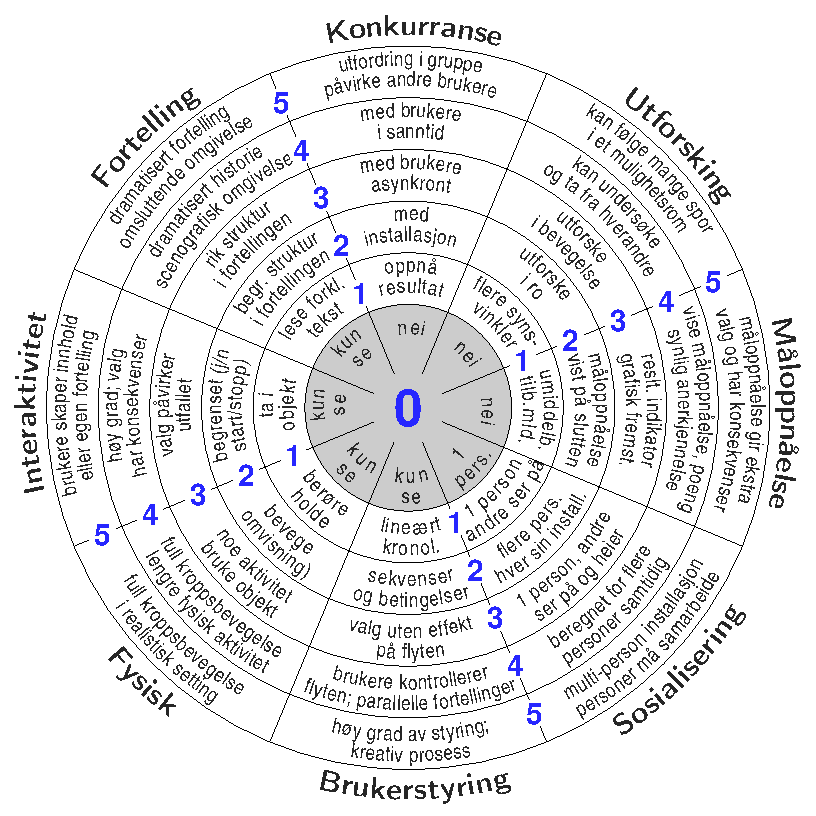
\includegraphics{figures/jVRARVestfold-ChartEPN}
\else
\begin{tikzpicture}[scale=1.75]
\path (\CNIPUSNL+\CNIPUSNLXX,\CNIPUSNL+\CNIPUSNLXX) --
(-\CNIPUSNL-\CNIPUSNLXX,\CNIPUSNL+\CNIPUSNLXX) --
(-\CNIPUSNL-\CNIPUSNLXX,-\CNIPUSNL-\CNIPUSNLXX) --
(\CNIPUSNL+\CNIPUSNLXX,-\CNIPUSNL-\CNIPUSNLXX);
% Draw background
\filldraw [fill=white!80!black] (0,0) circle (\CNIPUSNR/\CNIPUSNU*2);
\CNIPUSNdrawL
\filldraw [white!80!black,fill=white!80!black] (0,0) circle (\CNIPUSNR/\CNIPUSNU*0.7);
\renewcommand*{\mytextstyle}{\sffamily\large\bfseries\color{black!85}}
\renewcommand*{\myareatextstyle}{\fontfamily{phv}\fontseries{mc}\selectfont\footnotesize\color{black!85}}
\renewcommand*{\mynumbertextstyle}{\fontfamily{phv}\fontseries{mc}\selectfont\large\bfseries\color{blue!85}}
\renewcommand{\CNIPUSNlabeladjustment}{-2.0mm}
\renewcommand{\CNIPUSNraise}{-0.8ex}
%\fontfamily{phv}\fontseries{mc}\selectfont
\CNIPUSNtext{xxx}{1}{Konkurranse}
\CNIPUSNtext{xxx}{2}{Fortelling}
\CNIPUSNtext{xxx}{3}{Interaktivitet}
\CNIPUSNtext{xxx}{4}{Fysisk}
\CNIPUSNtext{xxx}{5}{Brukerstyring}
\CNIPUSNtext{xxx}{6}{Sosialisering}
\CNIPUSNtext{xxx}{7}{M{\aa}loppn{\aa}else}
\CNIPUSNtext{xxx}{8}{Utforsking}

% Competition
%\CNIPUSNareatext{xxx}{1}{{---}}{0}
\CNIPUSNareatext{xxx}{1}{nei}{0.2}
%1
\CNIPUSNareatext{xxx}{1}{oppn{\aa}}{1.4}
\CNIPUSNareatext{xxx}{1}{resultat}{1.0}
%2
\CNIPUSNareatext{xxx}{1}{med}{2.4}
\CNIPUSNareatext{xxx}{1}{installasjon}{2.0}
%3
\CNIPUSNareatext{xxx}{1}{med brukere}{3.4}
\CNIPUSNareatext{xxx}{1}{asynkront}{3.0}
%4
\CNIPUSNareatext{xxx}{1}{med brukere}{4.4}
\CNIPUSNareatext{xxx}{1}{i sanntid}{4.0}
%5
\CNIPUSNareatext{xxx}{1}{utfordring i gruppe}{5.4}
\CNIPUSNareatext{xxx}{1}{p{\aa}virke andre brukere}{5.0}

% Narrative
\CNIPUSNareatext{xxx}{2}{kun}{0.4}
\CNIPUSNareatext{xxx}{2}{se}{-0.0}
%1
\CNIPUSNareatext{xxx}{2}{lese forkl.}{1.4}
\CNIPUSNareatext{xxx}{2}{tekst}{1.0}
%2
\CNIPUSNareatext{xxx}{2}{begr.\ struktur}{2.4}
\CNIPUSNareatext{xxx}{2}{i fortellingen}{2.0}
%3
\CNIPUSNareatext{xxx}{2}{rik struktur}{3.4}
\CNIPUSNareatext{xxx}{2}{i fortellingen}{3.0}
%4
\CNIPUSNareatext{xxx}{2}{dramatisert historie}{4.4}
\CNIPUSNareatext{xxx}{2}{scenografisk omgivelse}{4.0}
%5
\CNIPUSNareatext{xxx}{2}{omsluttende omgivelse}{5.0}
\CNIPUSNareatext{xxx}{2}{dramatisert fortelling}{5.4}

% Interaction
\CNIPUSNareatext{xxx}{3}{kun}{0.4}
\CNIPUSNareatext{xxx}{3}{se}{-0.0}
%1
\CNIPUSNareatext{xxx}{3}{ta i}{1.4}
\CNIPUSNareatext{xxx}{3}{objekt}{1.0}
%2
\CNIPUSNareatext{xxx}{3}{begrenset (j/n}{2.4}
\CNIPUSNareatext{xxx}{3}{start/stopp)}{2.0}
%3
\CNIPUSNareatext{xxx}{3}{valg p{\aa}virker}{3.4}
\CNIPUSNareatext{xxx}{3}{utfallet}{3.0}
%4
\CNIPUSNareatext{xxx}{3}{h{\o}y grad; valg}{4.4}
\CNIPUSNareatext{xxx}{3}{har konsekvenser}{4.0}
%5
\CNIPUSNareatext{xxx}{3}{eller egen fortelling}{5.0}
\CNIPUSNareatext{xxx}{3}{brukere skaper innhold}{5.4}

% Physical
\CNIPUSNareatext{xxx}{4}{kun}{0.0}
\CNIPUSNareatext{xxx}{4}{se}{0.4}
%1
\CNIPUSNareatext{xxx}{4}{ber{\o}re}{1.0}
\CNIPUSNareatext{xxx}{4}{holde}{1.4}
%2
\CNIPUSNareatext{xxx}{4}{bevege}{2.0}
\CNIPUSNareatext{xxx}{4}{omvisning)}{2.4}
%3
\CNIPUSNareatext{xxx}{4}{noe aktivitet}{3.0}
\CNIPUSNareatext{xxx}{4}{bruke objekt}{3.4}
%4
\CNIPUSNareatext{xxx}{4}{full kroppsbevegelse}{4.0}
\CNIPUSNareatext{xxx}{4}{lengre fysisk aktivitet}{4.4}
%5
\CNIPUSNareatext{xxx}{4}{full kroppsbevegelse}{5.0}
\CNIPUSNareatext{xxx}{4}{i realistisk setting}{5.4}

% User Control
\CNIPUSNareatext{xxx}{5}{kun}{0.0}
\CNIPUSNareatext{xxx}{5}{se}{0.4}
%1
\CNIPUSNareatext{xxx}{5}{line{\ae}rt}{1.0}
\CNIPUSNareatext{xxx}{5}{kronol.}{1.4}
%2
\CNIPUSNareatext{xxx}{5}{sekvenser}{2.0}
\CNIPUSNareatext{xxx}{5}{og betingelser}{2.4}
%3
\CNIPUSNareatext{xxx}{5}{valg uten effekt}{3.0}
\CNIPUSNareatext{xxx}{5}{p{\aa} flyten}{3.4}
%4
\CNIPUSNareatext{xxx}{5}{brukere kontrollerer}{4.0}
\CNIPUSNareatext{xxx}{5}{flyten; parallelle fortellinger}{4.4}
%5
\CNIPUSNareatext{xxx}{5}{h{\o}y grad av styring;}{5.0}
\CNIPUSNareatext{xxx}{5}{kreativ prosess}{5.4}


% Social
\CNIPUSNareatext{xxx}{6}{1}{0.0}
\CNIPUSNareatext{xxx}{6}{pers.}{0.4}
%1
\CNIPUSNareatext{xxx}{6}{1 person}{1.0}
\CNIPUSNareatext{xxx}{6}{andre ser p{\aa}}{1.4}
%2
\CNIPUSNareatext{xxx}{6}{flere pers.}{2.0}
\CNIPUSNareatext{xxx}{6}{hver sin install.}{2.4}
%3
\CNIPUSNareatext{xxx}{6}{1 person, andre}{3.0}
\CNIPUSNareatext{xxx}{6}{ser p{\aa} og heier}{3.4}
%4
\CNIPUSNareatext{xxx}{6}{beregnet for flere}{4.0}
\CNIPUSNareatext{xxx}{6}{personer samtidig}{4.4}
%5
\CNIPUSNareatext{xxx}{6}{multi-person installasjon}{5.0}
\CNIPUSNareatext{xxx}{6}{personer m{\aa} samarbeide}{5.4}

% Achievements
%\CNIPUSNareatext{xxx}{7}{{---}}{0}
\CNIPUSNareatext{xxx}{7}{nei}{0.2}
%\CNIPUSNareatext{xxx}{7}{look}{0.4}
%\CNIPUSNareatext{xxx}{7}{only}{-0.1}
%1
\CNIPUSNareatext{xxx}{7}{umiddelb.}{1.4}
\CNIPUSNareatext{xxx}{7}{tilb.mld.}{1.0}
%2
\CNIPUSNareatext{xxx}{7}{m{\aa}loppn{\aa}else}{2.4}
\CNIPUSNareatext{xxx}{7}{vist p{\aa} slutten}{2.0}
%3
\CNIPUSNareatext{xxx}{7}{reslt. indikator}{3.4}
\CNIPUSNareatext{xxx}{7}{grafisk fremst.}{3.0}
%4
\CNIPUSNareatext{xxx}{7}{vise m{\aa}loppn{\aa}else, poeng}{4.4}
\CNIPUSNareatext{xxx}{7}{synlig anerkjennelse}{4.0}
%5
\CNIPUSNareatext{xxx}{7}{m{\aa}loppn{\aa}else gir ekstra}{5.4}
\CNIPUSNareatext{xxx}{7}{valg og har konsekvenser}{5.0}

% Explore
%\CNIPUSNareatext{xxx}{8}{{---}}{0}
%\CNIPUSNareatext{xxx}{8}{persp.}{0.4}
%\CNIPUSNareatext{xxx}{8}{fast}{0.0}
\CNIPUSNareatext{xxx}{8}{nei}{0.2}
%1
\CNIPUSNareatext{xxx}{8}{flere syns-}{1.4}
\CNIPUSNareatext{xxx}{8}{vinkler}{1.0}
%2
\CNIPUSNareatext{xxx}{8}{utforske}{2.4}
\CNIPUSNareatext{xxx}{8}{i ro}{2.0}
%3
\CNIPUSNareatext{xxx}{8}{utforske}{3.4}
\CNIPUSNareatext{xxx}{8}{i bevegelse}{3.0}
%4
\CNIPUSNareatext{xxx}{8}{kan unders{\o}ke}{4.4}
\CNIPUSNareatext{xxx}{8}{og ta fra hverandre}{4.0}
%5
\CNIPUSNareatext{xxx}{8}{kan f{\o}lge mange spor}{5.4}
\CNIPUSNareatext{xxx}{8}{i et mulighetsrom}{5.0}


\CNIPUSNNumbersL{3}
\CNIPUSNNumbersL{7}
\CNIPUSNNumbersL{1}
\CNIPUSNNumbersL{5}
%\filldraw [fill=white!80!black] (0,0) circle (\CNIPUSNR/\CNIPUSNU*1);
%\draw (0,0) node {0--5};
\node at (0,0)
%      [circle,inner sep=0pt, minimum size=0.4em,draw=white,fill=white]
      {\mynumbertextstyle\huge 0};
\end{tikzpicture}
\fi
%\end{center}
\caption{\EP{en} forklart med korte definisjoner; oversatt til norsk
  %fra engelsk original \citep{jLifSci16v8n12} 
  og tilpasset kunst i offentlige rom. 
  For å bestemme en verdi, søk etter nummer for beskrivelsen som
  passer best.}\label{fig:engagementprofile:n}
\end{figure}

\begin{figure}
\centering

\ifx\USETIKZINFIGURE\undefined
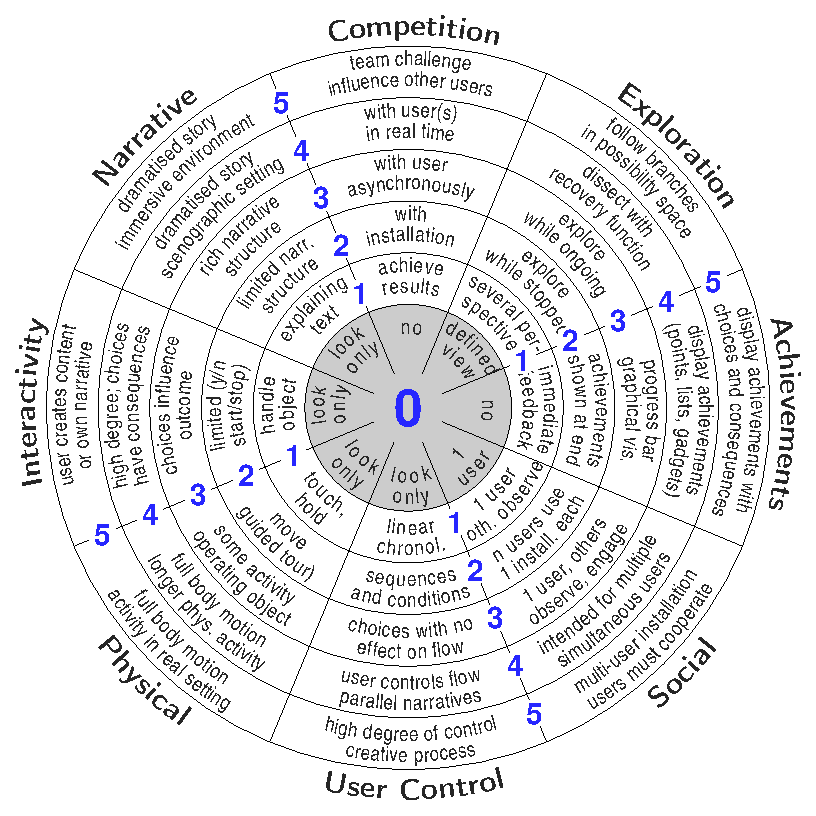
\includegraphics{figures/jVRARVestfold-ChartEPE}
\else
\begin{tikzpicture}[scale=1.75]
\path (\CNIPUSNL+\CNIPUSNLXX,\CNIPUSNL+\CNIPUSNLXX) --
(-\CNIPUSNL-\CNIPUSNLXX,\CNIPUSNL+\CNIPUSNLXX) --
(-\CNIPUSNL-\CNIPUSNLXX,-\CNIPUSNL-\CNIPUSNLXX) --
(\CNIPUSNL+\CNIPUSNLXX,-\CNIPUSNL-\CNIPUSNLXX);
% Draw background
\filldraw [fill=white!80!black] (0,0) circle (\CNIPUSNR/\CNIPUSNU*2);
\CNIPUSNdrawL
\filldraw [white!80!black,fill=white!80!black] (0,0) circle (\CNIPUSNR/\CNIPUSNU*0.7);
\renewcommand*{\mytextstyle}{\sffamily\large\bfseries\color{black!85}}
\renewcommand*{\myareatextstyle}{\fontfamily{phv}\fontseries{mc}\selectfont\footnotesize\color{black!85}}
\renewcommand*{\mynumbertextstyle}{\fontfamily{phv}\fontseries{mc}\selectfont\large\bfseries\color{blue!85}}
\renewcommand{\CNIPUSNlabeladjustment}{-2.0mm}
\renewcommand{\CNIPUSNraise}{-0.8ex}
%\fontfamily{phv}\fontseries{mc}\selectfont
\CNIPUSNtext{xxx}{1}{Competition}
\CNIPUSNtext{xxx}{2}{Narrative}
\CNIPUSNtext{xxx}{3}{Interactivity}
\CNIPUSNtext{xxx}{4}{Physical}
\CNIPUSNtext{xxx}{5}{User Control}
\CNIPUSNtext{xxx}{6}{Social}
\CNIPUSNtext{xxx}{7}{Achievements}
\CNIPUSNtext{xxx}{8}{Exploration}

% Competition
%\CNIPUSNareatext{xxx}{1}{{---}}{0}
\CNIPUSNareatext{xxx}{1}{no}{0.2}
%1
\CNIPUSNareatext{xxx}{1}{achieve}{1.4}
\CNIPUSNareatext{xxx}{1}{results}{1.0}
%2
\CNIPUSNareatext{xxx}{1}{with}{2.4}
\CNIPUSNareatext{xxx}{1}{installation}{2.0}
%3
\CNIPUSNareatext{xxx}{1}{with user}{3.4}
\CNIPUSNareatext{xxx}{1}{asynchronously}{3.0}
%4
\CNIPUSNareatext{xxx}{1}{with user(s)}{4.4}
\CNIPUSNareatext{xxx}{1}{in real time}{4.0}
%5
\CNIPUSNareatext{xxx}{1}{team challenge}{5.4}
\CNIPUSNareatext{xxx}{1}{influence other users}{5.0}

% Narrative
\CNIPUSNareatext{xxx}{2}{look}{0.4}
\CNIPUSNareatext{xxx}{2}{only}{-0.0}
%1
\CNIPUSNareatext{xxx}{2}{explaining}{1.4}
\CNIPUSNareatext{xxx}{2}{text}{1.0}
%2
\CNIPUSNareatext{xxx}{2}{limited narr.}{2.4}
\CNIPUSNareatext{xxx}{2}{structure}{2.0}
%3
\CNIPUSNareatext{xxx}{2}{rich narrative}{3.4}
\CNIPUSNareatext{xxx}{2}{structure}{3.0}
%4
\CNIPUSNareatext{xxx}{2}{dramatised story}{4.4}
\CNIPUSNareatext{xxx}{2}{scenographic setting}{4.0}
%5
\CNIPUSNareatext{xxx}{2}{immersive environment}{5.0}
\CNIPUSNareatext{xxx}{2}{dramatised story}{5.4}

% Interaction
\CNIPUSNareatext{xxx}{3}{look}{0.4}
\CNIPUSNareatext{xxx}{3}{only}{-0.0}
%1
\CNIPUSNareatext{xxx}{3}{handle}{1.4}
\CNIPUSNareatext{xxx}{3}{object}{1.0}
%2
\CNIPUSNareatext{xxx}{3}{limited (y/n}{2.4}
\CNIPUSNareatext{xxx}{3}{start/stop)}{2.0}
%3
\CNIPUSNareatext{xxx}{3}{choices influence}{3.4}
\CNIPUSNareatext{xxx}{3}{outcome}{3.0}
%4
\CNIPUSNareatext{xxx}{3}{high degree; choices}{4.4}
\CNIPUSNareatext{xxx}{3}{have consequences}{4.0}
%5
\CNIPUSNareatext{xxx}{3}{or own narrative}{5.0}
\CNIPUSNareatext{xxx}{3}{user creates content}{5.4}

% Physical
\CNIPUSNareatext{xxx}{4}{look}{0.0}
\CNIPUSNareatext{xxx}{4}{only}{0.4}
%1
\CNIPUSNareatext{xxx}{4}{touch,}{1.0}
\CNIPUSNareatext{xxx}{4}{hold}{1.4}
%2
\CNIPUSNareatext{xxx}{4}{move}{2.0}
\CNIPUSNareatext{xxx}{4}{guided tour)}{2.4}
%3
\CNIPUSNareatext{xxx}{4}{some activity}{3.0}
\CNIPUSNareatext{xxx}{4}{operating object}{3.4}
%4
\CNIPUSNareatext{xxx}{4}{full body motion}{4.0}
\CNIPUSNareatext{xxx}{4}{longer phys. activity}{4.4}
%5
\CNIPUSNareatext{xxx}{4}{full body motion}{5.0}
\CNIPUSNareatext{xxx}{4}{activity in real setting}{5.4}

% User Control
\CNIPUSNareatext{xxx}{5}{look}{0.0}
\CNIPUSNareatext{xxx}{5}{only}{0.4}
%1
\CNIPUSNareatext{xxx}{5}{linear}{1.0}
\CNIPUSNareatext{xxx}{5}{chronol.}{1.4}
%2
\CNIPUSNareatext{xxx}{5}{sequences}{2.0}
\CNIPUSNareatext{xxx}{5}{and conditions}{2.4}
%3
\CNIPUSNareatext{xxx}{5}{choices with no}{3.0}
\CNIPUSNareatext{xxx}{5}{effect on flow}{3.4}
%4
\CNIPUSNareatext{xxx}{5}{user controls flow}{4.0}
\CNIPUSNareatext{xxx}{5}{parallel narratives}{4.4}
%5
\CNIPUSNareatext{xxx}{5}{high degree of control}{5.0}
\CNIPUSNareatext{xxx}{5}{creative process}{5.4}


% Social
\CNIPUSNareatext{xxx}{6}{1}{0.0}
\CNIPUSNareatext{xxx}{6}{user}{0.4}
%1
\CNIPUSNareatext{xxx}{6}{1 user}{1.0}
\CNIPUSNareatext{xxx}{6}{oth.~observe}{1.4}
%2
\CNIPUSNareatext{xxx}{6}{n users use}{2.0}
\CNIPUSNareatext{xxx}{6}{1 install.~each}{2.4}
%3
\CNIPUSNareatext{xxx}{6}{1 user, others}{3.0}
\CNIPUSNareatext{xxx}{6}{observe, engage}{3.4}
%4
\CNIPUSNareatext{xxx}{6}{intended for multiple}{4.0}
\CNIPUSNareatext{xxx}{6}{simultaneous users}{4.4}
%5
\CNIPUSNareatext{xxx}{6}{multi-user installation}{5.0}
\CNIPUSNareatext{xxx}{6}{users must cooperate}{5.4}

% Achievements
%\CNIPUSNareatext{xxx}{7}{{---}}{0}
\CNIPUSNareatext{xxx}{7}{no}{0.2}
%\CNIPUSNareatext{xxx}{7}{look}{0.4}
%\CNIPUSNareatext{xxx}{7}{only}{-0.1}
%1
\CNIPUSNareatext{xxx}{7}{immediate}{1.4}
\CNIPUSNareatext{xxx}{7}{feedback}{1.0}
%2
\CNIPUSNareatext{xxx}{7}{achievements}{2.4}
\CNIPUSNareatext{xxx}{7}{shown at end}{2.0}
%3
\CNIPUSNareatext{xxx}{7}{progress bar}{3.4}
\CNIPUSNareatext{xxx}{7}{graphical vis.}{3.0}
%4
\CNIPUSNareatext{xxx}{7}{display achievements}{4.4}
\CNIPUSNareatext{xxx}{7}{(points, lists, gadgets)}{4.0}
%5
\CNIPUSNareatext{xxx}{7}{display achievements with}{5.4}
\CNIPUSNareatext{xxx}{7}{choices and consequences}{5.0}

% Explore
%\CNIPUSNareatext{xxx}{8}{{---}}{0}
\CNIPUSNareatext{xxx}{8}{defined}{0.4}
\CNIPUSNareatext{xxx}{8}{view}{0.0}
%1
\CNIPUSNareatext{xxx}{8}{several per-}{1.4}
\CNIPUSNareatext{xxx}{8}{spectives}{1.0}
%2
\CNIPUSNareatext{xxx}{8}{explore}{2.4}
\CNIPUSNareatext{xxx}{8}{while stopped}{2.0}
%3
\CNIPUSNareatext{xxx}{8}{explore}{3.4}
\CNIPUSNareatext{xxx}{8}{while ongoing}{3.0}
%4
\CNIPUSNareatext{xxx}{8}{dissect with}{4.4}
\CNIPUSNareatext{xxx}{8}{recovery function}{4.0}
%5
\CNIPUSNareatext{xxx}{8}{follow branches}{5.4}
\CNIPUSNareatext{xxx}{8}{in possibility space}{5.0}


\CNIPUSNNumbersL{3}
\CNIPUSNNumbersL{7}
\CNIPUSNNumbersL{1}
\CNIPUSNNumbersL{5}
%\filldraw [fill=white!80!black] (0,0) circle (\CNIPUSNR/\CNIPUSNU*1);
%\draw (0,0) node {0--5};
\node at (0,0)
%      [circle,inner sep=0pt, minimum size=0.4em,draw=white,fill=white]
      {\mynumbertextstyle\huge 0};
\end{tikzpicture}
\fi
%\end{center}
\caption{The dimensions of the \EP explained with short
  definitions. To define the value of a property, find the adjacent
  number of the phrases that fit best.}\label{fig:engagementprofile}
\end{figure}


\subsection{Indicator for Universal Design of AR/VR Installations}
%%%%%%%%%%%%%%%%%%%%%%%%%%%%%%%%%%%%%%%%%%%%%%%%%%%%%%%%%%%%%%%%%%%%%%%%%%%%%%%%
%%%%%%%%%%%%%%%%%%%%%%%%%%%%%%%%%%%%%%%%%%%%%%%%%%%%%%%%%%%%%%%%%%%%%%%%%%%%%%%%

%%%%%%%%%%%%%%%%%%%%%%%%%%%%%%%%%%%%%%%%%%%%%%%%%%%%%%%%%%%%%%%%%%%%%%%%%%%%%%%%%%%
%%%%%%%%%%%
%%%%%%%%%%% DIMENSION UUMUS example
\begin{figure}
\centering

\ifx\USETIKZINFIGURE\undefined
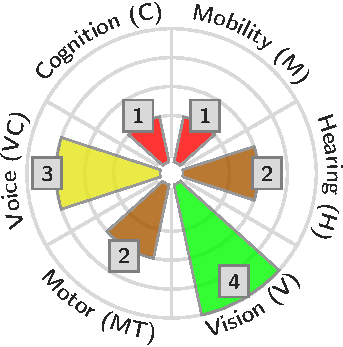
\includegraphics{figures/jVRARVestfold-UUMUS}
\else
\begin{tikzpicture}[scale=0.70]

\renewcommand{\UUMUSfontsize}{\small}
\renewcommand{\UUMUSareafontsize}{\small}
\renewcommand{\UUMUSnumberfontsize}{\small}
%\renewcommand{\UUMUSlabeladjustment}{-0.5mm}
%\renewcommand{\UUMUSraise}{-1.0ex}
\renewcommand{\UUMUSraise}{-0.5ex}

\path (\UUMUSL+\UUMUSLXX+2mm,\UUMUSL+\UUMUSLXX+2.5mm) --
(-\UUMUSL-\UUMUSLXX-2mm,\UUMUSL+\UUMUSLXX+2.5mm) --
(-\UUMUSL-\UUMUSLXX-2mm,-\UUMUSL-\UUMUSLXX-2.5mm) --
(\UUMUSL+\UUMUSLXX+2mm,-\UUMUSL-\UUMUSLXX-2.5mm);

% Draw background
\UUMUSdraw
% Draw labels
\UUMUStext{xxx}{1}{Cognition (C)}
\UUMUStext{xxx}{2}{Voice (VC)}
\UUMUStext{xxx}{3}{Motor (MT)}
\UUMUStext{xxx}{4}{Vision (V)}
\UUMUStext{xxx}{5}{Hearing (H)}
\UUMUStext{xxx}{6}{Mobility (M)}

% Draw in sector 1
\foreach \X in {1,2,...,6}{%
%\UUMUSdrawfill{fill=black}{\X}{0}
%\UUMUSdrawfill{fill=black!25!white}{\X}{3}
}

%\UUMUSfillborder{color=black!40!white, opacity=0.5}{1}{3}{3} % 0-ring
%\UUMUSfillarea{pattern=north east lines, pattern color=brown!60!black}{1}{2}{3} 
%\UUMUSline{color=orange,line width=2pt}{1}{3}
%\UUMUSdrawfill{fill=white!40!blue}{1}{0} % 

% Draw in sector 1C
%\UUMUSfillareanarrow{color=red!99!green, opacity=0.9}{1}{0}{1} 
\UUMUSuumus{1}{1}
%\UUMUSlabelbox{1}{1}{1}

% Draw in sector 2S
%\UUMUSfillareanarrow{color=red!66!green, opacity=0.9}{2}{0}{2} 
\UUMUSuumus{2}{3}

% Draw in sector 3M
%\UUMUSfillareanarrow{color=yellow!66!green, opacity=0.9}{3}{0}{3} 
\UUMUSuumus{3}{2}

% Draw in sector 4V
%\UUMUSfillareanarrow{color=red!1!green, opacity=0.9}{4}{0}{4} 
\UUMUSuumus{4}{4}

% Draw in sector 5H
%\UUMUSfillareanarrow{color=red!99!green, opacity=0.9}{5}{0}{1} 
\UUMUSuumus{5}{2}

% Draw in sector 6M
%\UUMUSfillareanarrow{color=red!99!green, opacity=0.9}{6}{0}{1} 
\UUMUSuumus{6}{1}


% colour formula: (value - 40) * 4
%\node at (0,{\UUMUSR/\UUMUSU*(1+1.4)}) {\mytextstyle -\,-}; 
%\node at (0,{\UUMUSR/\UUMUSU*(2+1.4)}) {\mytextstyle -}; 
%\node at (0,{\UUMUSR/\UUMUSU*(3+1.4)}) {\mytextstyle 0}; 
%\node at (0,{\UUMUSR/\UUMUSU*(4+1.4)}) {\mytextstyle +}; 
%\node at (0,{\UUMUSR/\UUMUSU*(5+1.4)}) {\mytextstyle ++}; 

\renewcommand{\UUMUSfontsize}{\scriptsize} % set to original value
\end{tikzpicture}
%
\fi
%
\caption{Eksempel UUMUS}
\label{fig:UUMUS:kunst}
\end{figure}
%%%%%%%%%%%%%%%%%%%%%%%%%%%%%%%%%%%%%%%%%%%%%%%%%%%%%%%%%%%%%%%%%%%%%%%%%%%%%%%%
%%%%%%%%%%%%%%%%%%%%%%%%%%%%%%%%%%%%%%%%%%%%%%%%%%%%%%%%%%%%%%%%%%%%%%%%%%%%%%%%


%%%%%%%%%%%%%%%%%%%%%%%%%%%%%%%%%%%%%%%%%%%%%%%%%%%%%%%%%%%%%%%%%%%%%%%%%%%%%%%%
%%%%%%%%%%%%%%%%%%%%%%%%%%%%%%%%%%%%%%%%%%%%%%%%%%%%%%%%%%%%%%%%%%%%%%%%%%%%%%%%


\citet{10.1007/978-3-030-29381-9-3} used accessibility indicators for
the assessment of science centre exhibits.
%\autocite[see also][]{NR-1042}. 
Their framework uses the following six indicator areas:
%\begin{enumerate*}[label={\alph*)},ref=\alph*]
%\item 
   vision (V), 
%\item 
   hearing (H), 
%\item 
   mobility (M), 
%\item 
   motor (MT), 
%\item 
   voice (VC), 
and 
%\item 
   cognition (C).
%\end{enumerate*}
Cognition, in turn, compounds a variety of processes, such as
orientation, language, reasoning, memory, concentration, coordination,
learning and engagement.

Their method quantifies the indicator areas into the following degrees of (in-)accessibility:
\begin{enumerate*}[label={\arabic*:},ref=\arabic*]
\item \emph{Indisputable/absolute barrier(s)} as showstoppers without work-around.
\item \emph{Significant barrier(s)} with significantly reduced user experience,
  increased time use, and increased risk for making mistakes. 
\item \emph{Minor barrier(s)} with a somewhat reduced user experience.
\item \emph{No barrier} providing normal user experience.
\end{enumerate*}
This scale is designed to have very few and comprehensible levels that
allow for quantifying different degrees of (in-)accessibility.

We suggest to adapt  this methodology to the use of AR/VR installations, and further develop it. 
We illustrate the use of this method with an example graph in \figurename~\ref{fig:UUMUS:kunst}.
\WVL{[missing: who is measuring/evaluating these, and how is communication of barriers done; this is an important research question for the VR/AR project]}


Some literature to check: 
\begin{itemize}
\item \url{https://doi.org/10.1016/j.compedu.2019.103778} (A systematic review of immersive virtual reality applications for higher education: Design elements, lessons learned, and research agenda)
\item \url{https://doi.org/10.3390/safety5030051} A Review of Virtual and Mixed Reality Applications in Construction Safety Literature H. Frank Moore and Masoud Gheisari 
\item \url{https://doi.org/10.1016/j.autcon.2017.11.003} ??? (A critical review of virtual and augmented reality (VR/AR) applications in construction safety) 
\item \url{https://doi.org/10.1080/10494820.2013.815221} ???
\item With uu, but maybe not what we want: \url{https://pdfs.semanticscholar.org/a77d/9ea21bbc94e6358ff8e7f1c0c4afa1336218.pdf}
\item With universal design for learning framework (UDL):  \url{https://doi.org/10.21125/inted.2019.1085} 
\item J. Beckmann, K. Menke, and P. Weber, “Universal Design for Learning in Augmented and Virtual Reality Trainings,” in Universal Access Through Inclusive Instructional Design: International Perspectives on UDL, S. L. Gronseth and E. M. Dalton, Eds.: Routledge, accepted and forthcoming in 2019. \url{https://doi.org/10.4324/9780429435515-39} har kun tilgang til google-preview. 
\item \url{https://doi.org/10.1145/3032970.3032981} ??? (Evaluating virtual reality and augmented reality training) tandfonline/ikke tilgang
\item \url{https://doi.org/10.1145/3234253.3234306} \dots ser relevant ut \dots inneholder en slags review på UX 
\end{itemize}

\subsection{From GB-ASSURE -- to be sorted}

\citet{rokhsaritalemiReviewMixedReality2020} stated that evaluating user satisfaction is critical to improve MR systems. Many researchers used surveys along parameters like fantasy, immersion, system feedback, cognitive load, user experience, gestural performance, etc. However, surveys are based on expressed subjectively, after the experience has taken place. 

\dots but some examples given in article; which variables to choose? Fantasy, immersion, system feedback; cognitive load, user experience, gestural performance; CPSS; \dots visualization; guidance, operation efficiency, operation complexity, operation precision, overall performance. … discussion about what parameters to use. 
Security aspects: probably not relevant here. 

Mixed reality survey: \citet{Costanza2009} \dots

This is some text about user experience, taken from previous work (ASSURE):

Users of data and services expect usable products that provide ease of use combined with good user experiences. This seems to be in conflict with these data and services being complex and distributed, and operating autonomously. The combination of complexity and user expectations is challenging the currently available methods that attempt to measure the degree of user experience. Further, it is challenging to increase the user experience of products or prototypes so that an effect can be documented.

Consumer products and services that do not provide sufficiently good user experiences will not be accepted by users and show low retention rates. That is, users will stop using these products or services that do not provide sufficient user experience (Clarke, Kinghorn, and et al. 2018). Insufficient user experience for subscription-based services or mobile apps can lead to products failing when these are refused by the (potential) users, for instance when the users are offered trial versions in an introductory phase.

User experience is influenced by seven factors that describe usefulness, usability, findability, credibility, desirability, accessibility, and value  (Interaction Design Foundation 2018). Good usability and accessibility is essential so that everyone is included in a world of ubiquitous data and services (United Nations 2006). Despite of legal obligations regarding accessibility, many products and services show insufficient user experience, specifically in terms of usability and accessibility (Kommunal- og Moderniseringsdepartementet 2013). 

Poor design of a product or service can limit groups with disabilities from taking part in the digital world \autocite{Bustard2013-gz} and result in loss of markets \autocite{Paz2016-vu}. As a countermeasure, design and assessment methods can be employed to create better design. For instance, \citet{aDesignProcess} presented an iterative design-methodology for installations in museums and science centres that incorporates continuous assessment during the development process.

Current assessment methods for user experience are often resource demanding, scale poorly, require expert knowledge, and can be inaccurate. For a world of ubiquitous data and services, including the Internet of Things (IoT), there is a need for a new generation of assessment tools better suited for distributed and networked systems. Herein, more accurate, consistent and automated methods have been requested by both the research community and the industry \autocite{Vermeeren2010-ub,Bai2016-ed,O_Shea2016-ll}. Checklist-based or survey-based methods are often used, but not sufficient in this context.

There is a variety of definitions for user experience (UX) that represent different perspectives and address elements such as focus, the experiencing agent, the object or artifact, how the experience is brought about, and the time of the experience \autocite{Law:2009:USD:1518701.1518813}. The international standard on ergonomics of human system interaction, ISO 9241-210 (International Standardization Organization 2010) defines user experience as "a person's perceptions and responses that result from the use or anticipated use of a product, system or service". According to this definition, user experience includes the users' emotions, beliefs, preferences, perceptions, physical and psychological responses, behaviour and accomplishments that occur before, during and after use. 
User experience evaluation and assessment (UXA) refers to a collection of methods, skills and tools utilised to uncover how a person perceives a system, before, during and after interacting with it. Assessment of user experience is non-trivial since user experience is subjective, context-dependent and dynamic over time. \citet{Vermeeren2010-ub} gave an overview of user experience evaluation methods.

New: look at this document: \citet{EGGER201935} \dots

Tbd. SUS and why other methods are necessary. \citet{brooke-1996} \dots Comments: \citet{tractinsky-usabilityconstruct}

\citet{martenssonPeerEngagementTeaching2016} presented a variety of definitions for engagement in an overview. 
\citet{Reeve2009} defined engagement as follows: “Engagement refers to the behavioural intensity and emotional quality of a person’s active involvement during a task.” 
\citet{lemkeDocumentingAssessingLearning2015} defined engagement as the “Affective involvement in and commitment to an activity, goal, practice, group, or community that enhances the quality and quantity of participation despite obstacles, setbacks, or frustrations; distinguished from enjoyment.”

The ASSURE vision is that with today’s increased collection and aggregation of data on user interaction with digital services there is an enormous potential for developing radically new techniques for assessment. Such methods can combine input from multiple sources, objective and subjective, to better understand user experience, and build better and more adaptive services. However, such methods can challenge privacy, as a person’s observed behaviour can reveal preferences. Multidisciplinary research combining the fields of ICT and IoT, machine learning, psychology, usability, and privacy is necessary for the development of such a framework.

When assessing how well a service or a product works, usually, methodologies such as checklists, user studies, questionnaires, observations, focus groups, etc. are used. As such assessment can be biased by a deviation between expressed and real experiences or by interpretations of an observer, we intend to use sensors that assess the users’ bio-physiological data and other measurable data. Further, for digital services and products, usage data from these services and products can be used. 


\subsection{Evaluation of Universal Design in General}

Universell utforming %\footnote{Takk til Kristin Skeide Fuglerud for
                     %en gjennomgang av dette avsnittet.} 
er påbudt gjennom Diskriminerings- og
tilgjengelighetsloven (DTL) \autocite{dtl-2013} og
vil være relevant også for utforming av VR/AR installasjoner til trening. 
\citet{kristins-phd} gir en oversikt over temaet universell utforming i sin avhandling.

Det finnes så langt ikke en enkel
utviklingsmetodikk som kan garantere for universelt utformet IKT,
men en brukersentrert utviklingsprosess har vist seg å være et godt
valg. 
I tillegg til at løsningen må overholde retningslinjer som f.eks.\ WCAG
2.1 \autocite{WCAG-21}, 
bør det gjennomføres utprøvinger der brukere med ulike behov
deltar, inkludert personer med funksjonsnedsettelser (sensoriske,
motoriske, kognitive).
Man kan også vurdere brukskvalitet
ved hjelp av validert spørreundersøkelse, som for eksempel
SUS \autocite{brooke-1996}. Vi viser også til et
eksempel fra et tidligere
prosjekt \autocite{schulz-gladhorn-saether-2015}.

%%%%%%%%%%%%%%%%%%%%%%%%%%%%%%%%%%%%%%%%%%%%%%%%%%%%%%%%%%%%%%%%%%%%%%%%%%%%%%%%
%%%%%%%%%%%%%%%%%%%%%%%%%%%%%%%%%%%%%%%%%%%%%%%%%%%%%%%%%%%%%%%%%%%%%%%%%%%%%%%%

\section{Konsept for studie med brukermedvirkning}

%Studien med brukermedvirkning består av to deler:
%\begin{enumerate*}[label={\arabic*)},ref=\arabic*]
%\item utforming og evaluering av spørreundersøkelse
%og
%\item utforming av veileder til fokusgruppe.
%\end{enumerate*}
For å studere forskningsspørsmålene kan det utarbeides spørreskjema til
medlemmer i målgruppen. 

\subsection{Spørreskjema via digital plattform}

Spørreskjemaer kan utarbeides via digital plattform, der svarene kan avgis anonymt.
Et eksempel er bruk av Google Forms \autocite{google-forms}.

Spørreskjemaenet kan deles inn i avdelinger med følgende innhold: 
\begin{enumerate*}[label={\alph*)},ref=\alph*]
\item spørsmål om bruk av AR/VR-installasjoner, vist i \tablename~\ref{tab:questions:m};
\item spørsmål om målgruppens IT-bruk, vist i \tablename~\ref{tab:questions:it};
\item spørsmål om funksjonalitet i en app, vist i \tablename~\ref{tab:questions:utforming};
\item spørsmål om engasjement (\ep{en}), vist i \tablename~\ref{tab:questions:opinion};
og
\item spørsmål om behov for tilrettelegging, vist i \tablename~\ref{tab:questions:uu}.
\end{enumerate*}

%\subsubsection{Temaer i spørreskjemaet}

Angående bruk av AR/VR-installasjoner var målet å kartlegge hvilke tilbud
som benyttes og hvordan disse benyttes. Spørreskjemaet inneholder
spørsmål om hvor ofte deltakerne benytter seg av \dots
Denne avdelingen
av spørreskjemaet er gjengitt i \tablename~\ref{tab:questions:m}.
\WVL{[spørreskjemaet må tilpasses; spørsmålene er fra et annet prosjekt]}

%%%%%%%%%%%%%%%%%%%%%%%%%%%%%%%%%%%%%%%%%%%%%%%%%%%%%%%%%%%%%%%%%%%%%%%%%%%%%%%%

\begin{sidewaystable}
    \caption{Formulering av spørsmålene om bruk av museer og kultur \WVL{[--- må endres]}.} \label{tab:questions:m}
\centering\small
\begin{tabular}{lp{.43\hsize}p{.43\hsize}}
 & Spørsmål & Svaralternativer \\
\hline
\(Q_{m1}\) & Bruker du museer?  & få ganger i året; en gang i måneden; flere ganger i måneden; ukentlig og mer\\
\(Q_{m2}\) & Har du brukt byguide?  & nei; prøvde, men det var ikke noe for meg; ja, ved behov\\
\(Q_{m3}\) & Har du brukt QR-kodene på Poesiparken? & nei; prøvde, men det var ikke noe for meg; ja\\
\(Q_{m4}\) & Oppsøker du kultur via digitale ressurser?  &nei; av og til; ja, ofte.\\
\(Q_{m5}\) & Skriv navn på digitale ressurser du oppsøkte  & fritekst\\
\(Q_{m6}\) & Har du brukt Kahoot!  & ja, bl.a.\ i selskapelig lag (julebord, firmafest); har sett noen bruke det (f.eks. barn eller barnebarn i skolesammenheng); nei, har ikke hørt om dette før nå.\\
\(Q_{m7}\) & Hvor mange kunstverk i offentlig rom kjenner du til i kommunen du bor i? Skriv et omtrent-tall:  & tallverdi \\
\(Q_{m8}\) & Har du eksempler på slik kunst? Nevn gjerne plassering, tittel eller kunstner.  & fritekst\\
\(Q_{m9}\) & Hva slags kunst i offentlig rom engasjerer? Beskriv kort:  & fritekst
\end{tabular}
\end{sidewaystable}

%%%%%%%%%%%%%%%%%%%%%%%%%%%%%%%%%%%%%%%%%%%%%%%%%%%%%%%%%%%%%%%%%%%%%%%%%%%%%%%%

%%%%%%%%%%%%%%%%%%%%%%%%%%%%%%%%%%%%%%%%%%%%%%%%%%%%%%%%%%%%%%%%%%%%%%%%%%%%%%%%

\begin{sidewaystable}
    \caption{Formulering av spørsmålene om IT-bruk \WVL{[--- må endres]}.} \label{tab:questions:it}
\centering\small
\begin{tabular}{lp{.43\hsize}p{.43\hsize}}
 & Spørsmål & Svaralternativer \\
\hline
\(Q_{it1}\) & Hva slags telefon bruker du til daglig?  & kun fasttelefon; kun fasttelefon, men jeg har nettbrett; mobiltelefon med taster; smart-telefon; annet \\
\(Q_{it2}\) & Bruker du nettbrett?  & nei (har ikke); av og til; ofte \\
\(Q_{it3}\) & Hvilken type smarttelefon eller nettbrett har du?  & iPhone/iPad; Android; WindowsPhone; annet; vet ikke\\
\(Q_{it4}\) &  Bruker du tjenester som AppStore eller GooglePlay for å laste ned innhold eller apper? & ja, ofte; 
ja, sjelden en gang; vet ikke hva dette er \\
\(Q_{it5}\) &  Har du laget en snarvei til en web-side på hjem-skjermen (på nettbrett eller
smarttelefon) & ja; nei; vet ikke hvordan dette gjøres; vet ikke hva dette er \\
\(Q_{it6}\) &  Bruker du trådløs sone (Wifi) med telefonen & ja; nei \\
\(Q_{it7}\) &  Bruker du datanettverk med telefonen (3G,4G) & ja; nei \\
\(Q_{it8}\) &  Bruker du Bluetooth til noe? & nei; kun til å høre musikk; ja \\
\(Q_{it9}\) &  Hva bruker du Bluetooth til & fritekst \\
\(Q_{it10}\) &  Hvor ofte bruker du digitale apper? & aldri; en gang i måneden; en gang i uken; en gang per dag; mange ganger per dag\\
\(Q_{it11}\) &  Angi apper som du pleier å bruke & fritekst \\
\(Q_{it12}\) &  Bruker du følgende tjenester (flere svar mulig)? & Vipps; telefonbank; nettbank \\
\(Q_{it13}\) &  Bruker du telefonen for å få informasjon når du er ute og reiser? & har ikke telefon med når jeg reise; kun for å ringe med; ja, med apper; annet \\
\(Q_{it14}\) &  Beskriv hvordan du bruker telefonen når du er ute og reiser & fritekst \\
\(Q_{it15}\) &  Har du brukt tjenester der din nåværende posisjon blir brukt? & nei; av og til; ja, ofte\\
\(Q_{it16}\) &  Har du brukt QR-kode? & nei; av og til; ja, ofte\\
\end{tabular}
\end{sidewaystable}

%%%%%%%%%%%%%%%%%%%%%%%%%%%%%%%%%%%%%%%%%%%%%%%%%%%%%%%%%%%%%%%%%%%%%%%%%%%%%%%%

\WVL{[må endres]}
I en undersøkelse vil man være interessert i detaljer for hvordan målgruppen
bruker mobiltelefon og nettbrett, hvilken plattform de har, hvilken
relevant funksjonalitet de bruker, og hvordan telefonen brukes når de
reiser.  Videre ble det tatt opp spørsmål om brukergruppens bruk av
nettverk (Wifi, WLAN, Bluetooth), sporings- og
identifiseringsteknologier (posisjonering, Bluetooth, QR-kode).
Denne avdelingen
av spørreskjemaet er gjengitt i \tablename~\ref{tab:questions:it}.
\WVL{[spørreskjemaet må tilpasses; det er andre bruksmønstre, 
f.eks.\ erfaringer med AR/VR vil være relevante. Spørsmålene i tabellen er fra et annet prosjekt]}


%%%%%%%%%%%%%%%%%%%%%%%%%%%%%%%%%%%%%%%%%%%%%%%%%%%%%%%%%%%%%%%%%%%%%%%%%%%%%%%%

\WVL{[må endres]}
Angående ønsket funksjonalitet av AR/VR installasjoner og apper vil man spørre om dette. 
Dette vil bestemmes av anvendelsesområde.
Denne avdelingen
av spørreskjemaet er gjengitt i \tablename~\ref{tab:questions:utforming}.
\WVL{[spørreskjemaet må tilpasses; 
anvendelsesområde, f.eks.\ fysisk trening, arbeidstrening, situasjonsforståelse, osv. vil være relevant.
Spørsmålene i tabellen er fra et annet prosjekt]}

%%%%%%%%%%%%%%%%%%%%%%%%%%%%%%%%%%%%%%%%%%%%%%%%%%%%%%%%%%%%%%%%%%%%%%%%%%%%%%%%

\begin{table}
    \caption{Formulering av spørsmålene om utforming \WVL{[--- må endres]}.} \label{tab:questions:utforming}
\centering\small
\begin{tabular}{lp{.9\hsize}}
\multicolumn{2}{p{.99\hsize}}{For hver av spørsmålene brukes følgende skala:}\\ 
\multicolumn{2}{p{.99\hsize}}{1=uenig, 2=delvis uenig, 3=verken enig eller uenig, 4=delvis enig, 5=enig.}\\
\hline
\(Q_{f1}\) & En app skal gi meg informasjon om et kunstverk i det offentlige rom når jeg ser det. \\
\(Q_{f2}\) & En app skal gjøre meg oppmerksom på et kunstverk i det offentlige rom når jeg er i
nærheten av det. \\
\(Q_{f3}\) & En app skal gi meg oversikt over alle kunstverk i et bestemt område. \\
\(Q_{f4}\) & En app skal vise meg veien til et kunstverk i det offentlige rom jeg velger ut. \\
\(Q_{f5}\) & En app skal gi meg fordypende materiale til et kunstverk, f.eks. video-filmer, lydforedrag,
lenke til bøker og litteratur.
\end{tabular}
\end{table}

%%%%%%%%%%%%%%%%%%%%%%%%%%%%%%%%%%%%%%%%%%%%%%%%%%%%%%%%%%%%%%%%%%%%%%%%%%%%%%%%

For å vurdere engasjement la vi engasjementsprofilen til
grunn. Vanligvis mil man la brukere prøve en prototyp og så spørre
om de ønsker mer eller mindre av en
egenskap. Da det ikke forelå en prototyp, spurte vi på generell basis
om de var enig eller uenig
i en av de åtte påstandene som er avledet vurderingsmetoden for
endringer i utviklingsrunder \autocite{aDesignProcess}.
Denne avdelingen
av spørreskjemaet er gjengitt i \tablename~\ref{tab:questions:opinion}.
\WVL{[spørreskjemaet må tilpasses til anvendelsesområde;
kun mindre tilpassing til anvendelsesområde; evt.\ erstatte ordet ``app'' med noe mer passende. 
Spørsmålene i tabellen er i utgangspunktet fra et annet prosjekt]}

%%%%%%%%%%%%%%%%%%%%%%%%%%%%%%%%%%%%%%%%%%%%%%%%%%%%%%%%%%%%%%%%%%%%%%%%%%%%%%%%
%%%%%%%%%%%%%%%%%%%%%%%%%%%%%%%%%%%%%%%%%%%%%%%%%%%%%%%%%%%%%%%%%%%%%%%%%%%%%%%%

\begin{table}
    \caption{Formulering av spørsmålene om engasjement \WVL{[--- må tilpasses]}.} \label{tab:questions:opinion}
\centering\small
\begin{tabular}{lp{.9\hsize}}
\multicolumn{2}{p{.99\hsize}}{Det brukes følgende skala for hvert av spørsmålene:}\\ 
\multicolumn{2}{p{.99\hsize}}{1=uenig, 2=delvis uenig, 3=verken enig eller uenig, 4=delvis enig, 5=enig.}\\
\hline
\(Q_C\) & En app skal tilby funksjonalitet for konkurranse, f.eks. quiz eller spill der man får poeng
og kan konkurrere med andre. \\
\(Q_N\) & En app skal bake presentasjonen inn i en lengre fortelling. \\
\(Q_I\) & En app skal gi deg individuelle tilbakemeldinger om \WVL{[tbd.]}. \\
\(Q_P\) &En app skal gi deg et utvalg av ulik grad av fysisk utfordring når du \WVL{[tbd.]}. \\
\(Q_U\) & En app skal la deg selv ta alle veivalg. Den skal ikke foreslå forhåndsbestemte opplegg \WVL{[tbd.]}. \\
\(Q_S\) & En app skal stimulere til sosiale aktiviteter med andre mennesker når du  \WVL{[tbd.]}. \\
\(Q_A\) & En app skal gi deg synlige bevis at du har oppnådd mål \WVL{[tbd.]}. \\
\(Q_E\) & En app skal gi deg mulighet å utforske \WVL{[tbd.]}.
\end{tabular}
\end{table}

%%%%%%%%%%%%%%%%%%%%%%%%%%%%%%%%%%%%%%%%%%%%%%%%%%%%%%%%%%%%%%%%%%%%%%%%%%%%%%%%
%%%%%%%%%%%%%%%%%%%%%%%%%%%%%%%%%%%%%%%%%%%%%%%%%%%%%%%%%%%%%%%%%%%%%%%%%%%%%%%%

Prinsippene for universell utforming burde gjelde for AR/VR trening.
I det tidligere prosjektet ble det spurt om  hvor stor behovet for tilrettelegging for
målgruppen (eldre) er med tanke på utfordringer som kan oppstå med
begrenset syn, hørsel, bruk av berøringskjerm og bruk av hjelpemidler
pga.\ redusert bevegelighet. Vi anmerker at prinsippene for universell
utforming gjelder selv om man adresserer disse spesifikke
problemstillingene særskilt. 
Denne avdelingen
av spørreskjemaet er gjengitt i \tablename~\ref{tab:questions:uu}.
\WVL{[spørreskjemaet må omarbeides fullstendig og adressere universell utforming på en mer egnet måte. 
F.eks.\ bruk av metode for å vurdere universell utforming i museer. I
det lille prosjektet det refereres til her var det ikke rom for en
større undersøkelse rundt dette. tbd.]}

%%%%%%%%%%%%%%%%%%%%%%%%%%%%%%%%%%%%%%%%%%%%%%%%%%%%%%%%%%%%%%%%%%%%%%%%%%%%%%%%

\begin{table}
    \caption{Formulering av spørsmålene om universell utforming \WVL{[--- må endres --- her kommer det helt forskjellige spørsmål]}.} \label{tab:questions:uu}
\centering\small
\begin{tabular}{lp{.9\hsize}}
\multicolumn{2}{p{.99\hsize}}{For hver av spørsmålene brukes følgende skala:}\\ 
\multicolumn{2}{p{.99\hsize}}{1=uenig, 2=delvis uenig, 3=verken enig eller uenig, 4=delvis enig, 5=enig.}\\
\hline
\(Q_{u1}\) & Jeg trenger tilrettelegging for innhold på skjermen.\\
\(Q_{u2}\) & Jeg trenger tilrettelegging for lyd-innhold.\\
\(Q_{u3}\) & Jeg trenger tilrettelegging for berøringskjerm\\
\(Q_{u4}\) & Jeg trenger tilrettelegging fordi jeg ikke kan bruke telefonen mens jeg går (f.eks.\ pga.\
rullator eller andre hjelpemidler)
\end{tabular}
\end{table}

%%%%%%%%%%%%%%%%%%%%%%%%%%%%%%%%%%%%%%%%%%%%%%%%%%%%%%%%%%%%%%%%%%%%%%%%%%%%%%%%


\subsection{Resultater fra spørreskjema}

 

%%%%%%%%%%%%%%%%%%%%%%%%%%%%%%%%%%%%%%%%%%%%%%%%%%%%%%%%%%%%%%%%%%%%%%%%%%%%%%%%
%%%%%%%%%%%%%%%%%%%%%%%%%%%%%%%%%%%%%%%%%%%%%%%%%%%%%%%%%%%%%%%%%%%%%%%%%%%%%%%%

\begin{table}
    \caption{Resultater fra spørsmålene \(Q_{f1} \dots Q_{f5}\) og
      spørsmålene om engasjement. \WVL{[dette er resultater fra et annet prosjekt -- vises kun som eksempel]}}\label{tab:results:2}
\centering\footnotesize

\begin{tabular}{l|ccccc|cccccccc}
      & \(Q_{f1}\) & \(Q_{f2}\) & \(Q_{f3}\) & \(Q_{f4}\) & \(Q_{f5}\) & \(Q_{C}\) & \(Q_{N}\)& \(Q_{I}\)& \(Q_{P}\)& \(Q_{U}\)& \(Q_{S}\) & \(Q_{A}\) & \(Q_{E}\) \\
\hline
mean & 4.09 &	3.78 &	3.96 &	4.19 &	3.72 &	2.63 &	2.77 &	2.87 &
2.66 &	3.24 &	3.03 &	2.23 &	4.11 \\
\(\sigma^2\) & 1.33 &	1.56 &	1.52 &	1.13 &	1.66 &	1.84 &	1.44 &
1.45 &	1.34 &	1.77 &	1.50 &	1.48 &	1.25  \\
\hline
90\% &  5 &	5 &	5 &	5 &	5 &	5 &	4 &	4.9 &	4 &	5 &	4.9 &	4 &	5 \\
med.  &  4 &	4 &	4 &	5 &	4 &	3 &	3 &	3 &	3 &	3 &	3 &	2 &	5 \\
10\% & 3 &	2 &	2.1 &	3 &	2 &	1 &	1 &	1 &	1 &	1 &	1 &	1 &	3 \\
\hline
\(+\)  &  75\%&	63\%&	71\%&	79\%&	58\%&	24\%&	25\%&	27\%&	18\%&	43\%&	38\%&	13\%&	71\%\\
0      &  16\%&	24\%&	19\%&	16\%&	28\%&	29\%&	38\%&	40\%&	44\%&	31\%&	34\%&	31\%&	22\%\\
\(-\)  &   9\%&	13\%&	11\%&	 5\%&	14\%&	46\%&	38\%&	33\%&	38\%&	26\%&	29\%&	56\%&	6\%\\
\hline
%ratio  & 3.64&	2.31&	3.03&	4.42&	2.04&	0.71&	0.83&	0.91&	0.75&	1.30&	1.14&	0.50&	3.28\\
\(r\)  & 4.89&	2.93&	3.98&	6.47&	2.56&	0.64\adfarrowse5&	0.78&	0.88&	0.66\adfarrowse5&	1.41\adfarrowne5&	1.20&	0.39\adfarrows5&	4.74\adfarrown5\\
%rekkefølge   & 2 & 4 & 3 & 1 & 5 & & & & & & & &   \\
%vurdering &   &   &   &   &   & \((-)\) & & & \((-)\) & \((+)\) & & \(-\)& \(+\)  

\end{tabular}
\end{table}

%%%%%%%%%%%%%%%%%%%%%%%%%%%%%%%%%%%%%%%%%%%%%%%%%%%%%%%%%%%%%%%%%%%%%%%%%%%%%%%%
%%%%%%%%%%%%%%%%%%%%%%%%%%%%%%%%%%%%%%%%%%%%%%%%%%%%%%%%%%%%%%%%%%%%%%%%%%%%%%%%


%%%%%%%%%%%%%%%%%%%%%%%%%%%%%%%%%%%%%%%%%%%%%%%%%%%%%%%%%%%%%%%%%%%%%%%%%%%%%%%%%%%
%%%%%%%%%%%
%%%%%%%%%%% 494 participants 10-percentili
\begin{figure}
\centering

\ifx\USETIKZINFIGURE\undefined
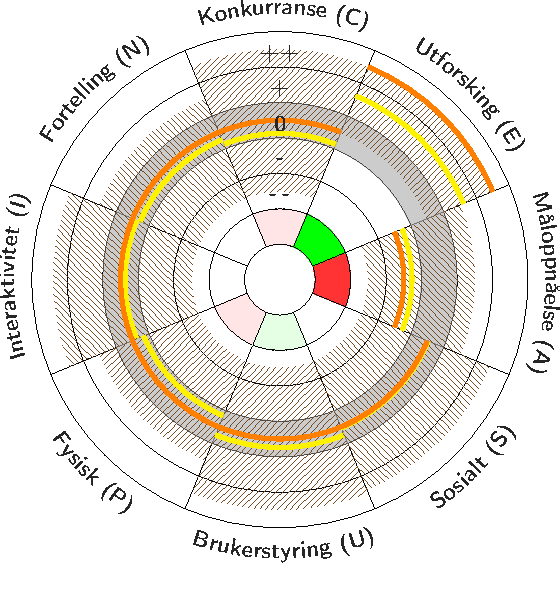
\includegraphics{figures/engagementikunior-112}
\else
\begin{tikzpicture}[scale=1.2]
\fontfamily{phv}\fontseries{mc}\selectfont
%\renewcommand{\CNIPUSNfontsize}{\normalsize}
\renewcommand{\CNIPUSNfontsize}{\small}
%\renewcommand*{\mytextstyle}{\fontfamily{phv}\fontseries{mc}\large\bfseries\color{black!85}}
%\renewcommand*{\myareatextstyle}{\fontfamily{phv}\fontseries{mc}\selectfont\footnotesize\color{black!85}}
%\renewcommand*{\mynumbertextstyle}{\fontfamily{phv}\fontseries{mc}\selectfont\large\bfseries\color{blue!85}}
\renewcommand{\CNIPUSNlabeladjustment}{-0.6mm}
\renewcommand{\CNIPUSNraise}{-0.5ex}

\path (\CNIPUSNL+\CNIPUSNLXX,\CNIPUSNL+\CNIPUSNLXX) --
(-\CNIPUSNL-\CNIPUSNLXX,\CNIPUSNL+\CNIPUSNLXX) --
(-\CNIPUSNL-\CNIPUSNLXX,-\CNIPUSNL-\CNIPUSNLXX-5mm) --
(\CNIPUSNL+\CNIPUSNLXX,-\CNIPUSNL-\CNIPUSNLXX-5mm);
%
% Draw background
\CNIPUSNdraw
% Draw labels
\CNIPUSNtext{xxx}{1}{Konkurranse (C)}
\CNIPUSNtext{xxx}{2}{Fortelling (N)}
\CNIPUSNtext{xxx}{3}{Interaktivitet (I)}
\CNIPUSNtext{xxx}{4}{Fysisk (P)}
\CNIPUSNtext{xxx}{5}{Brukerstyring (U)}
\CNIPUSNtext{xxx}{6}{Sosialt (S)}
\CNIPUSNtext{xxx}{7}{M{\aa}loppn{\aa}else (A)}
\CNIPUSNtext{xxx}{8}{Utforsking (E)}

% Draw in sector 1
\foreach \X in {1,2,...,8}{%
%\CNIPUSNdrawfill{fill=black}{\X}{0}
%\CNIPUSNdrawfill{fill=black!25!white}{\X}{3}
}

% Draw in sector 1C
\CNIPUSNfillborder{color=black!40!white, opacity=0.5}{1}{3}{3} % 0-ring
\CNIPUSNfillarea{pattern=north east lines, pattern color=brown!60!black}{1}{1}{5} % 3..4
\CNIPUSNline{color=yellow,line width=2pt}{1}{2.63}
\CNIPUSNline{color=orange,line width=2pt}{1}{3}
\CNIPUSNdrawfill{fill=white!90!red}{1}{0} 
%\CNIPUSNdrawfill{fill=white!1!green}{1}{0} % 43
% Formula: (x - 20)*3

% Draw in sector 2N
\CNIPUSNfillborder{color=black!40!white, opacity=0.5}{2}{3}{3} % 0-ring
\CNIPUSNfillarea{pattern=north west lines, pattern color=brown!60!black}{2}{1}{4} % 3..4
\CNIPUSNline{color=yellow,line width=2pt}{2}{2.77}
\CNIPUSNline{color=orange,line width=2pt}{2}{3}
%\CNIPUSNdrawfill{fill=white!20!blue}{2}{0}
%\CNIPUSNdrawfill{fill=white!84!green}{2}{0} % 61

% Draw in sector 3I
\CNIPUSNfillborder{color=black!40!white, opacity=0.5}{3}{3}{3} % 0-ring
\CNIPUSNfillarea{pattern=north west lines, pattern color=brown!60!black}{3}{1}{4.9} % 2.5 .. 4
\CNIPUSNline{color=yellow,line width=2pt}{3}{2.87}
\CNIPUSNline{color=orange,line width=2pt}{3}{3}
%\CNIPUSNdrawfill{fill=white!20!blue}{3}{0}
%\CNIPUSNdrawfill{fill=white!44!green}{3}{0} % 51

% Draw in sector 4P
\CNIPUSNfillborder{color=black!40!white, opacity=0.5}{4}{3}{3} % 0-ring
\CNIPUSNfillarea{pattern=north east lines, pattern color=brown!60!black}{4}{1}{4} % 3 .. 5
\CNIPUSNline{color=yellow,line width=2pt}{4}{2.66}
\CNIPUSNline{color=orange,line width=2pt}{4}{3}
\CNIPUSNdrawfill{fill=white!90!red}{4}{0}
%\CNIPUSNdrawfill{fill=white!1!green}{4}{0} % 40

% Draw in sector 5U
\CNIPUSNfillborder{color=black!40!white, opacity=0.5}{5}{3}{3} % 0-ring
\CNIPUSNfillarea{pattern=north east lines, pattern color=brown!60!black}{5}{1}{5} % 3 .. 5
\CNIPUSNline{color=orange,line width=2pt}{5}{3}
\CNIPUSNline{color=yellow,line width=2pt}{5}{3.24}
\CNIPUSNdrawfill{fill=white!90!green}{5}{0} % 47
%\CNIPUSNdrawfill{fill=white!28!green}{5}{0} % 47

% Draw in sector 6S
\CNIPUSNfillborder{color=black!40!white, opacity=0.5}{6}{3}{3} % 0-ring
\CNIPUSNfillarea{pattern=north west lines, pattern color=brown!60!black}{6}{1}{4.9} % 2 .. 4
\CNIPUSNline{color=yellow,line width=2pt}{6}{3.03}
\CNIPUSNline{color=orange,line width=2pt}{6}{3}
%\CNIPUSNdrawfill{fill=white!20!blue}{6}{0} 
%\CNIPUSNdrawfill{fill=white!84!green}{6}{0} % 61

% Draw in sector 7A
\CNIPUSNfillborder{color=black!40!white, opacity=0.5}{7}{3}{3} % 0-ring
\CNIPUSNfillarea{pattern=north west lines, pattern color=brown!60!black}{7}{1}{4} % 3 .. 4
\CNIPUSNline{color=orange,line width=2pt}{7}{2}
\CNIPUSNline{color=yellow,line width=2pt}{7}{2.23}
\CNIPUSNdrawfill{fill=white!20!red}{7}{0} 
%\CNIPUSNdrawfill{fill=white!32!green}{7}{0} % 48

% Draw in sector 8E
\CNIPUSNfillborder{color=black!40!white, opacity=0.5}{8}{3}{3} % 0-ring
\CNIPUSNfillarea{pattern=north east lines, pattern color=brown!60!black}{8}{3}{5} % 3 .. 4
\CNIPUSNline{color=orange,line width=2pt}{8}{5}
\CNIPUSNline{color=yellow,line width=2pt}{8}{4.11}
\CNIPUSNdrawfill{fill=white!1!green}{8}{0} % 61
%\CNIPUSNdrawfill{fill=white!84!green}{8}{0} % 61

%%all cyan lines
%\CNIPUSNline{color=cyan, line width=2pt}{1}{3.66}
%\CNIPUSNline{color=cyan, line width=2pt}{2}{3.26}
%\CNIPUSNline{color=cyan, line width=2pt}{3}{3.38}
%\CNIPUSNline{color=cyan, line width=2pt}{4}{3.65}
%\CNIPUSNline{color=cyan, line width=2pt}{5}{3.50}
%\CNIPUSNline{color=cyan, line width=2pt}{6}{3.19}
%\CNIPUSNline{color=cyan, line width=2pt}{7}{3.43}
%\CNIPUSNline{color=cyan, line width=2pt}{8}{3.30}



% colour formula: (value - 40) * 4

\node at (0,{\CNIPUSNR/\CNIPUSNU*(1+1.4)}) {\mytextstyle -\,-}; 
\node at (0,{\CNIPUSNR/\CNIPUSNU*(2+1.4)}) {\mytextstyle -}; 
\node at (0,{\CNIPUSNR/\CNIPUSNU*(3+1.4)}) {\mytextstyle 0}; 
\node at (0,{\CNIPUSNR/\CNIPUSNU*(4+1.4)}) {\mytextstyle +}; 
\node at (0,{\CNIPUSNR/\CNIPUSNU*(5+1.4)}) {\mytextstyle ++}; 

\renewcommand{\CNIPUSNfontsize}{\scriptsize} % set to original value

%\CNIPUSNnumbers{1}
\end{tikzpicture}
\fi

\caption{%
Engasjementsdiagram for app / digital plattform for
kunst i offentlige rom;
112 deltakere i aldersgruppen 60+. 
Skraveringer representerer svarene mellom 10\% og  90\%
percentilene; orange linjer: median-verdi; gule linjer: middelverdi.
Segmentene i midten viser om deltakerne {\o}nsker (gr{\o}nn) eller ikke
{\o}nsker (r{\o}dt) disse elementene.
\WVL{[dette er resultater fra et annet prosjekt -- vises kun som eksempel]}
}%
\label{fig:Opinion:112}
\end{figure}
%%%%%%%%%%%%%%%%%%%%%%%%%%%%%%%%%%%%%%%%%%%%%%%%%%%%%%%%%%%%%%%%%%%%%%%%%%%%%%%%
%%%%%%%%%%%%%%%%%%%%%%%%%%%%%%%%%%%%%%%%%%%%%%%%%%%%%%%%%%%%%%%%%%%%%%%%%%%%%%%%

%label: fig:Opinion:112


%%%%%%%%%%%%%%%%%%%%%%%%%%%%%%%%%%%%%%%%%%%%%%%%%%%%%%%%%%%%%%%%%%%%%%%%%%%%%%%%
%%%%%%%%%%%%%%%%%%%%%%%%%%%%%%%%%%%%%%%%%%%%%%%%%%%%%%%%%%%%%%%%%%%%%%%%%%%%%%%%

\begin{table}
    \caption{Resultater fra spørsmålene om spesifikke behov for
      utforming (\(Q_{u1} \dots Q_{u4}\)). \WVL{[dette er resultater fra et annet prosjekt -- vises kun som eksempel]}}\label{tab:results:3}
\centering\small

\begin{tabular}{l|cccc}
      &  \(Q_{u1}\) & \(Q_{u2}\) & \(Q_{u3}\) & \(Q_{u4}\) \\
\hline
mean & 	2.89 &	2.88 &	2.59 &	1.73 \\
\(\sigma^2\) &	2.30 &	2.20 &	2.19 & 1.32 \\
\hline
90\% &  5 &	5 &	5 &	3\\
med.  & 	3 &	3 & 3 & 1\\
10\% & 	1 &	1 &	1 &	1\\
\hline
\(+\)  & 	35\%&	32\%&	27\%&	8\%\\
0      &	29\%&	34\%&	27\%&	19\%\\
\(-\)  &        36\%&	35\%&	45\%&	72\%\\

\end{tabular}
\end{table}

%%%%%%%%%%%%%%%%%%%%%%%%%%%%%%%%%%%%%%%%%%%%%%%%%%%%%%%%%%%%%%%%%%%%%%%%%%%%%%%%
%%%%%%%%%%%%%%%%%%%%%%%%%%%%%%%%%%%%%%%%%%%%%%%%%%%%%%%%%%%%%%%%%%%%%%%%%%%%%%%%


%%%%%%%%%%%%%%%%%%%%%%%%%%%%%%%%%%%%%%%%%%%%%%%%%%%%%%%%%%%%%%%%%%%%%%%%%%%%%%%%
%\begin{figure}
%\centering
%\includegraphics[width=.48\hsize]{figures/ikunior-chart-fu}
%\
%\includegraphics[width=.48\hsize]{figures/ikunior-chart-uu}
%\caption{graph 1}\label{fig:diagram:fu}
%\end{figure}
%%%%%%%%%%%%%%%%%%%%%%%%%%%%%%%%%%%%%%%%%%%%%%%%%%%%%%%%%%%%%%%%%%%%%%%%%%%%%%%%

I en evaluering vil vi bruke følgende vurderingsmetode:
Vi beregner forholdet \(r\) mellom positive og negative besvarelser som
følger, der \(p\) beskriver antall positive, \(n\) antall negative og \(z\) antall nøytrale besvarelser; \(f\) er en vekt-faktor, f.eks. 0.5: \(r=\frac{p+f\cdot z}{n+f\cdot z}\).
Terskelverdier for \(r\) settes som følger: \(<0.55\)
sterk negativ (rødt);  \(<0.75\) noe negativ; \(>1.30\) noe
positiv;  \(>1.75\) sterk positiv (grønn); ellers nøytral. Dersom det
er mer enn 50\% nøytral settes det blå farge. Dersom det er veldig få
som stemmer nøytralt, må man gjøre særskilte vurderinger fordi
opinionen er splittet i slike tilfeller. 
Diagram for engasjement er vist i \figurename~\ref{fig:Opinion:112}.


\WVL{[dette er et eksempel for en vurdering, gjennomført for tidligere prosjekt; beskrivelse må tilpasses.]}
Angående parametre om engasjement ble det gjort følgende funn: 
\begin{enumerate*}[label={\alph*)},ref=\alph*]
\item appen skal gi mulighet for \emph{å utforske på egenhånd}; 
\item det er \emph{ikke noe ønske om synlige bevis} for at de har besøkt kunst i
offentlig rom (altså ikke noen slags {\textquotedblleft}elektroniske
pins{\textquotedblright}); 
\item de ønsker å styre besøket sitt selv og
dermed \emph{ikke ha ferdiglagde opplegg}; 
\item de stiller seg svakt
negativ til konkurranser; 
\item de stiller seg nøytralt til sosial
aktivitet; og 
\item de stiller seg nøytralt til svakt negativ til
fortelling, interaktivitet og fysisk aktivitet. 
Denne informasjonen kan gi gode innspill til hva som skal prioriteres
samt om utformingen av app.
\end{enumerate*}

\WVL{[Dette er resultater fra et tidligere prosjekt. Dette er kun ment som illustrasjon på et tidligere resultat.]}
Resultater for spørsmålene om universell utforming er vist i \tablename~\ref{tab:results:3}.
Angående universell utforming: Ca $\frac13$ ønsker tilrettelegging,
$\frac13$ stiller seg nøytral, og $\frac13$ trenger ikke
tilrettelegging for det visuelle, det auditive og berøringskjerm. Det ser
ikke ut til å være et særskilt behov for å tilrettelegge for bruken av
app mens man er i bevegelse. Det bemerkes at kravene til universell
utforming gjelder og at appen må være tilrettelagt til at alle i
målgruppen kan bruke den, ifølge lovverket. 
%Se eget avsnitt om
%universell utforming senere i dokumentet.


%%%%%%%%%%%%%%%%%%%%%%%%%%%%%%%%%%%%%%%%%%%%%%%%%%%%%%%%%%%%%%%%%%%%%%%%%%%%%%%%
%%%%%%%%%%%%%%%%%%%%%%%%%%%%%%%%%%%%%%%%%%%%%%%%%%%%%%%%%%%%%%%%%%%%%%%%%%%%%%%%
%
%%%%%%%%%%%%%%%%%%%%%%%%%%%%%%%%%%%%%%%%%%%%%%%%%%%%%%%%%%%%%%%%%%%%%%%%%%%%%%%%%%%%
%%%%%%%%%%%
%%%%%%%%%%% DIMENSION UUMUS example
\begin{figure}
\centering

\ifx\USETIKZINFIGURE\undefined
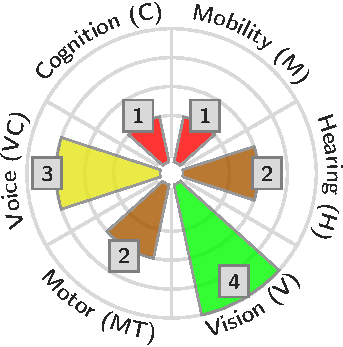
\includegraphics{figures/jVRARVestfold-UUMUS}
\else
\begin{tikzpicture}[scale=0.70]

\renewcommand{\UUMUSfontsize}{\small}
\renewcommand{\UUMUSareafontsize}{\small}
\renewcommand{\UUMUSnumberfontsize}{\small}
%\renewcommand{\UUMUSlabeladjustment}{-0.5mm}
%\renewcommand{\UUMUSraise}{-1.0ex}
\renewcommand{\UUMUSraise}{-0.5ex}

\path (\UUMUSL+\UUMUSLXX+2mm,\UUMUSL+\UUMUSLXX+2.5mm) --
(-\UUMUSL-\UUMUSLXX-2mm,\UUMUSL+\UUMUSLXX+2.5mm) --
(-\UUMUSL-\UUMUSLXX-2mm,-\UUMUSL-\UUMUSLXX-2.5mm) --
(\UUMUSL+\UUMUSLXX+2mm,-\UUMUSL-\UUMUSLXX-2.5mm);

% Draw background
\UUMUSdraw
% Draw labels
\UUMUStext{xxx}{1}{Cognition (C)}
\UUMUStext{xxx}{2}{Voice (VC)}
\UUMUStext{xxx}{3}{Motor (MT)}
\UUMUStext{xxx}{4}{Vision (V)}
\UUMUStext{xxx}{5}{Hearing (H)}
\UUMUStext{xxx}{6}{Mobility (M)}

% Draw in sector 1
\foreach \X in {1,2,...,6}{%
%\UUMUSdrawfill{fill=black}{\X}{0}
%\UUMUSdrawfill{fill=black!25!white}{\X}{3}
}

%\UUMUSfillborder{color=black!40!white, opacity=0.5}{1}{3}{3} % 0-ring
%\UUMUSfillarea{pattern=north east lines, pattern color=brown!60!black}{1}{2}{3} 
%\UUMUSline{color=orange,line width=2pt}{1}{3}
%\UUMUSdrawfill{fill=white!40!blue}{1}{0} % 

% Draw in sector 1C
%\UUMUSfillareanarrow{color=red!99!green, opacity=0.9}{1}{0}{1} 
\UUMUSuumus{1}{1}
%\UUMUSlabelbox{1}{1}{1}

% Draw in sector 2S
%\UUMUSfillareanarrow{color=red!66!green, opacity=0.9}{2}{0}{2} 
\UUMUSuumus{2}{3}

% Draw in sector 3M
%\UUMUSfillareanarrow{color=yellow!66!green, opacity=0.9}{3}{0}{3} 
\UUMUSuumus{3}{2}

% Draw in sector 4V
%\UUMUSfillareanarrow{color=red!1!green, opacity=0.9}{4}{0}{4} 
\UUMUSuumus{4}{4}

% Draw in sector 5H
%\UUMUSfillareanarrow{color=red!99!green, opacity=0.9}{5}{0}{1} 
\UUMUSuumus{5}{2}

% Draw in sector 6M
%\UUMUSfillareanarrow{color=red!99!green, opacity=0.9}{6}{0}{1} 
\UUMUSuumus{6}{1}


% colour formula: (value - 40) * 4
%\node at (0,{\UUMUSR/\UUMUSU*(1+1.4)}) {\mytextstyle -\,-}; 
%\node at (0,{\UUMUSR/\UUMUSU*(2+1.4)}) {\mytextstyle -}; 
%\node at (0,{\UUMUSR/\UUMUSU*(3+1.4)}) {\mytextstyle 0}; 
%\node at (0,{\UUMUSR/\UUMUSU*(4+1.4)}) {\mytextstyle +}; 
%\node at (0,{\UUMUSR/\UUMUSU*(5+1.4)}) {\mytextstyle ++}; 

\renewcommand{\UUMUSfontsize}{\scriptsize} % set to original value
\end{tikzpicture}
%
\fi
%
\caption{Eksempel UUMUS}
\label{fig:UUMUS:kunst}
\end{figure}
%%%%%%%%%%%%%%%%%%%%%%%%%%%%%%%%%%%%%%%%%%%%%%%%%%%%%%%%%%%%%%%%%%%%%%%%%%%%%%%%
%%%%%%%%%%%%%%%%%%%%%%%%%%%%%%%%%%%%%%%%%%%%%%%%%%%%%%%%%%%%%%%%%%%%%%%%%%%%%%%%

%
%%%%%%%%%%%%%%%%%%%%%%%%%%%%%%%%%%%%%%%%%%%%%%%%%%%%%%%%%%%%%%%%%%%%%%%%%%%%%%%%
%%%%%%%%%%%%%%%%%%%%%%%%%%%%%%%%%%%%%%%%%%%%%%%%%%%%%%%%%%%%%%%%%%%%%%%%%%%%%%%%


\subsubsection{State of the art}

\subsubsection{Knowledge needs and project objectives}
Participatory design and co-creation are considered to be some of the best methods for understanding a target audience
and creating high quality, well designed solutions to meet their needs and preferences. Despite this, several reviews
conclude that the user-involvement in the design and development of e-health services is
insufficient\footnote{Sosial- og helsedepartementet (2001). Fra bruker til borger. En strategi for nedbygging av
funksjonshemmende barrierer. Oslo.}, \autocite{manzoorEservicesSocialInclusion2017a}, and needs to be strengthened\footnote{\ Forskningsrådet. Evaluering av
samhandlingsreformen: sluttrapport fra styringsgruppen for forskningsbasert følgeevaluering av samhandlingsreformen
(EVASAM). Oslo: Forskningsrådet; 2016.}. Moreover, research that develop and evaluate digital health services designed
for people with disabilities, seldom include people with disabilities in the study sample \autocite{10.3389/fpsyg.2018.02323,10.1007/978-3-319-58634-2_15}.

Despite the benefits documented in the scientific literature of XR developed for special user groups, such assistive
technology (AT) has very low uptake and high abandonment rates \autocite{schererWhyPeopleUse2015}.
Thus, assistive technology targeted at small user groups has a very limited potential for increasing equity and
reducing exclusion of vulnerable user groups. Some important reasons for the low uptake and high abandonment rates
could be that a) people with disabilities are often omitted from the research and development process b) the lack of
collaboration between end-users, researchers, and developers in industry c) the lack of policy platforms to support the
translation of prototype conceptualization in research to actual implementation in the community and d) lack of
sustainable business models when the target user groups are small. Also, while studies do report positive effects for
special user groups, it is difficult to generalise from a limited number of participants to larger groups. 

This project will develop a framework with accompanying tools that can be used to evaluate whether XR installations
(hardware and software) are accessible, usable, and suitable for users with various needs and abilities, and to put
forward requirements for such technology. The framework and tools can be used by organisations that acquire or develop
VR/AR to integrate accessibility as early as possible and thus contribute to equal opportunities for people and larger
audiences for VR/AR solutions.

In the second step we will, in cooperation with organisations and industry, create a reference architecture and find and
adapt accessibility plugins, that can be integrated in existing or new XR technology to make them more accessible. 

When people use XR technology, they are presented with a scenario (i.e., a sequence of events in an
environment)\footnote{Simulation Interoperability Standards Organization. SISO-GUIDE-006-2018 – Guideline on
Scenario Development for Simulation Environments, 2018; Siegfried R, Laux A, Rother M et al. Scenarios in
military (distributed) simulation environments. In Proc. 2012 Spring Simulation Interoperability Workshop.
12S-SIW-014.}. The basic idea is that scenarios should be described digitally in a machine-readable format.
Furthermore, there should be enough information in this description for the scenario to be presented in different
modalities that can be adapted to people with different abilities. The digital scenario description is thus universally
designed, while individual adaptations are made at the presentation level. 

This requires a loose coupling between the scenario as such and how the scenario is implemented in various mixed reality
platforms (Unity, Unreal, VBS, etc.). The project will develop a reference architecture\footnote{The Open Group: SOA
Reference Architecture Technical Standard (2011), doc. no. C119} \autocite{hannay-vandenBerg-NATO-2017}
for universally designed digital scenarios as described
above. A reference architecture is a design template, which systems developers can use when implementing solutions.
Adhering to this reference architecture should ensure that solutions embody the stated principles for universal design
and adaptations to particular user groups. Figure 1 outlines the idea of this reference architecture. The project will
focus on what information digital scenarios must contain to be universally designed (green artefact in the middle), as
well as to find out how the information can be used in different mixed-reality platforms to implement adaptations to
different users (green boxes on the right). The balance between generic and customization-specific information will be
a central theme.

Figure 1 \WVL{[tbd.]} also shows how a system that uses universally designed digital scenarios is intended to be used. Healthcare
professionals should be able to design scenarios in an easy-to-understand tool 
\autocite{10.1007/978-3-030-50732-9_60,Hannay2019StructuredCT}, 
and a scenario generator will represent the scenario digitally, together with any scoring models to
measure relevant aspects during plays \autocite{DashleyK.RouwendalvanSchijndel_etal2020}. 
When the scenario is run on different mixed reality
platforms with different adaptations, events and changes in the environment is largely determined by a joint event
manager and a stage \& content manager, respectively (ibid). 

\subsection{Research questions and hypotheses, theoretical approach and methodology}
Main hypotheses: 

\begin{enumerate}
\item It is possible to create a framework with accompanying tools that will enable developers to create more
accessible, inclusive, universally designed mainstream XR solutions. These created solutions will reach beyond the
target groups of users with disabilities. We will reach additional target groups like for example the elderly or people
who are situationally disabled by employing more flexible and adaptable techniques. Finally, we will contribute to
reduce inequality of XR-based health and welfare services. 
\item When presenting user needs in a systematic form, the goals and purposes of universal design of XR, together with
concrete ideas and solutions for specific accessibility challenges, and offer empirical evaluation and testing with end
users together with partners in the health sector and industry will seize the opportunity and implement accessibility
features into some of their solutions.
\end{enumerate}
\subsubsection[\ Research questions: ]{\ Research questions: }
\begin{itemize}
\item What type of co-creation methods can be used to enhance the voice of users and stakeholders in the different
stages of the problem-solving process? 

\begin{itemize}
\item What type of XR are considered important/interesting for Enthusiast target users. 
\item What features are important for accessibility and user experience? 
\item When is XR appropriate for Enthusiast target users? When is it not?
\item What are the benefits and limitations of XR in health and welfare related training scenarios for our target
groups?
\end{itemize}
\item What are the characterizing factors of universally designed XR solutions and how can the degree of accessibility
and engagement for various user groups be described and measured? 

\begin{itemize}
\item What criteria are important for an inclusive user experience of XR?
\item What other frameworks can be used as a basis for developing our framework (universal design for learning,
engagement profiles, universal design in other contexts, e.g. museums)?
\end{itemize}
\end{itemize}
\begin{itemize}
\item \begin{itemize}
\item How can we measure accessibility and user experience? (e.g. through observations, measurements, etc.? Can sensors,
Brain Computing Interface (BCI) or other tools be used for automatic evaluation of the user experience – as a
supplement to empirical evaluation methods? \ 
\item How can our framework and accessibility be used by software/hardware producers and their customers to create more
inclusive XR systems? What are concrete recommendations for hardware manufacturers and software developers.
\end{itemize}
\end{itemize}
\begin{itemize}
\item How can we define a reference architecture that allows XR manufacturers to integrate accessibility plugins into
their mainstream XR? 

\begin{itemize}
\item Which aspects should be covered by the universally designed digital scenario, and which aspects should be covered
by the specific adaptations to different user groups (Figure 1)? For example, should engagement principles be stated as
part of the universally designed scenario or as part of the adaptations. 
\item How well does the reference architecture accommodate state-of-practice and possibly proprietary stove-piped
solutions; hereunder,

\begin{itemize}
\item What types of accessibility objects/plugins exists and how are they integrated with \ \ mainstream XR? 
\item How feasible is it that industry will adhere to the reference architecture ideal? 
\end{itemize}
\item What is the user experience of users with disabilities of the adapted solution? 
\end{itemize}
\end{itemize}
\begin{itemize}
\item How can municipal, industry and other stakeholder be educated and engaged in the promotion of universal design of
XR? 
\end{itemize}
\subsubsection{Theoretical approach and methodology}
Co-creation describes an interaction where actors jointly produce a mutually valued outcome based on their assessments
of the risks and benefits of the proposed courses of action, and decisions based on dialogue, access to information and
resources, as well as transparency\footnote{\ Prahalad, C. K., \& Ramaswamy, V. (2004). Co-creation experiences: The
next practice in value creation. Journal of Interactive Marketing, 18(3), 5-14. doi:https://doi.org/10.1002/dir.20015
}. Co-creation has the potential to reduce siloed-working. It may refer to any act of collective creativity, i.e.
creativity that is shared by two or more people\footnote{Sanders, E.B.N. \& P.J. Stappers. (2008) Co-creation and the
new landscapes of design. CoDesign. 4(1):5-18.}. Co-creational approaches including actively involving intended users
has increasingly been applied to redesigning health services,\footnote{Chamberlain, P. \& R. Partridge
(2017). Co-designing co-design. Shifting the culture of practice in healthcare. The Design
Journal. 20 (sup. 1):2010-2021}. In this project we define co-creation pragmatically as creative, open and participatory
and inclusive processes aiming at a) identifying user needs, b) exploring, building and sharing knowledge, ideas and
concerns across organisational roles and cultures, and c) making the iterative minor and major adjustments necessary
for reaching the strategic research goals and to develop accompanying and practical tools\footnote{Dugstad, J., et
al. (2018), Towards successful implementation of digital night monitoring technology through co-creation. A four-year
longitudinal case-study}.


\subsubsection{Interdisciplinary consideration and cooperation}
The proposal brings together organisations and individuals in a unique interdisciplinary and cross-sectional
collaboration in rehabilitation research in Norway and beyond. Building on the network of the project partners and the
reference group we will reach out to national and international stakeholders. This will further strengthen the network
between service users in municipality and research in the implementation and use of XR technology in the health and
welfare sector to ensure equity and equality to health and welfare services.

\subsubsection[\ Ethical considerations]{\ Ethical considerations}
Close collaboration with stakeholders will ensure RRI (Responsible research \& innovation). As the project involves
vulnerable groups, ethical aspects will be considered during all stages of the project. Further, ethical considerations
will be systematically integrated into the co-creation and evaluation processes. All participation by stakeholders and
users will be regulated by informed consent. To address ethical aspects related to the use of XR as health technology,
we will use the Morally Relevant Questions with Respect to Assessing Health Technology introduced by 
\citet{hofmann_droste_oortwijn_cleemput_sacchini_2014}
%Hofmann et al.
%(2014)\footnote{\ Hofmann, B., Droste, S., Oortwijn, W., Cleemput, I., \& Sacchini, D. (2014). Harmonization of ethics in health technology assessment: a revision of the Socratic approach. International journal of technology assessment in health care, 30(1), 3.} 
including 33 questions within seven domains. 
What are\dots: 
\begin{enumerate*}[label={\arabic*.\ },ref=\arabic*]
\item \dots the morally relevant issues related
to the diagnosis and the patient group? 
\item \dots the ethical, social, cultural, legal, and religious challenges related to
the health technology? 
\item \dots the moral challenges with structural changes related to the health technology? 
\item \dots the moral
issues related to the characteristics of the health technology? 
\item \dots the moral issues related to stakeholders? 
\item \dots the
moral issues related to the assessment of the health technology? 
\item Are there additional moral issues?
\end{enumerate*}

\subsection[Novelty and ambition ]{Novelty and ambition }
That the universally designed scenarios do not have to be implemented time and time again for each new adaptation, and
that adaptations are made only in the mixed-reality platforms, is a loose coupling in line with the concept Modelling
\& Simulation as Service (MSaaS\footnote{\ van den Berg, T.W., Huiskamp, W., Siegfried, R., Lloyd, J., Grom, A.,
Phillips, R.: Modelling and Simulation as a Service: Rapid deployment of interoperable and credible simulation
environments – an overview of NATO MSG-136. In: Proc. 2018 Winter Simulation Innovation Workshop. No. 18W-SIW-018
(2018)}[FFFC?] . This concept is essential for enabling universally designed solutions for different user groups
quickly. The flexibility in this is also necessary for rapid testing and evaluation of solutions.

The anticipated results are both theoretical and practical:
\begin{enumerate}
\item 
A survey and overview of challenges and opportunities of VR for people with disabilities. 
This milestone has as overall goal to raise awareness and deepen the understanding of accessibility in VR.

\item An assessment tool to evaluate the accessibility of VR systems, hardware, software, etc. with respect to the
dimensions of cognition, mobility, hearing, vision, motor, and/or voice. In this milestone, we will provide a
checklist or some other half-automated tool that can be used by manufacturers, developers and customers of VR systems
to evaluate the accessibility of any given VR system.

\item A survey of existing tools and solutions to address some of the challenges discovered in the previous milestones. We
will list and review plugins, hardware, development frameworks, and provide some suggestions on how to compensate for
some of the challenges that people with impairment(s) might face.

\item A specification on how to make VR systems more accessible for people with disabilities.
The outcome of this milestone will be a list of recommendations and concrete specifications that manufacturers and
developers can use to create well-rounded and universally designed VR system.

\item An empirical evaluation with actual user groups connected to our partners (most likely the deaf and/or people with
autism).
We will verify the ENTHUSIAST framework empirically with one/two concrete user groups: from the assessment of existing
games and setups, suggestions on how to improve them, implementations of our specifications (in form of plugins,
add-ons, extra-hardware, etc), to the evaluation of accessibility and perceived engagement before and after
accessibility improvement.
\end{enumerate}

\section[Impact ]{Impact }
\subsection[Potential impact of the proposed research ]{Potential impact of the proposed research }
There are several outputs from the project. First there is the UD-XR evaluation and development framework. This will
describe accessibility needs and requirements for a broad range of user groups, and with detail and emphasis on the
needs of the user groups in our partner organisations. Secondly, there will a solution architecture with a set of
accessibility features that can be implemented. 

With the advancing commercial feasibility, ongoing popularity and omnipresent digitalisation of public and official
life, it is very probable that there are going to be more legal requirements to digital accessibility which includes
VR/AR/MR21, similar to for example the 2019 European Accessibility
Act\footnote{https://eur-lex.europa.eu/legal-content/EN/TXT/?uri=uriserv:OJ.L\_.2019.151.01.0070.01.ENG\&toc=OJ:L:2019:151:TOC
\ } and the Norwegian Equality and Anti-Discrimination Act\footnote{https://lovdata.no/dokument/NLE/lov/2017-06-16-51}.
The UN Convention on the Rights of Persons with Disabilities aims to ensure that disabled people can enjoy the full
range of human rights: civil, political, economic, social, and cultural. This shall, among other things, be ensured
through requirements for accessible ICT (Article 2). The Convention refers to the concept of universal design (UD) as a
means through which to achieve this goal (Article 4). 

As in the web accessibility domain there will be need for assistive technology (AT), specially designed for certain user
groups. However, integrating accessibility as a fundamental core part of a mainstream XR-system will be valuable not
only for people with disabilities, but also to create a more flexible, adaptive and inclusive technology ecosystem that
will benefit a wide range of users, such as people of different ages, languages, and everyone experiences situational
disabilities dependent on their context21. Universally designed mainstream technology has many advantages over
specialized technology, such as lower cost, increased availability, and creating equal opportunities and social
acceptability. 





%\newpage
%ACKNOWLEDGMENTS are optional
\paragraph{Takk.}
%\textsl{
\WVL{[tbd]}

Arbeidet som er presentert her ble gjennomført i prosjektet
\WVL{[tbd]} finansiert av
\WVL{[tbd]}
%
Deler av forskningen ble støttet gjennom basisfinansiering for
institutter hos Norsk Regnesentral, prosjektnummer 194067 i Norges
Forskningsråd.


\paragraph{Forfatterbidragene.}
\WVL{[tbd]}

\paragraph{Interessekonflikter.}
\WVL{[tbd]}

%\bibliographystyle{plain}
%\bibliographystyle{plainnat}
%\bibliographystyle{chicago}
%\bibliography{visitorengagement,seriousgames,extended-reality}
\printbibliography

%\appendix
%\input{Vedlegg-E-Intervjuguide-IKUNIOR}

\end{document}
